\DeclareUnicodeCharacter{2212}{-}
\DeclareUnicodeCharacter{223C}{-}

\documentclass[natbib]{muthesis_tawat_alex}
\usepackage{natbib}
%\usepackage[numbers,square]{natbib}


% if you are not using the author-year ref system remove [natbib]
% from the above line
% IMPORTANT!!! -- DO NOT USE THIS FILE FOR YOUR THESIS --
% INSTEAD make a COPY of it and call it something like mythesis.tex
% i.e. cp -i muthesis_temlate.tex mythesis.tex
%\usepackage{cite}
\usepackage{lscape}
\usepackage{svg}
%\draft
% in draft mode there is one title page (title, candidate, abstract)
% no tables of contents, etc or
%\notitlepage  % (only works in draft mode)
% put your own newcommands and calls to packages here
\usepackage{graphicx} % for input of graphics files
\usepackage{amsmath,amssymb} % for improved equation formating and symbols
\usepackage{subfig} %for figures
\usepackage{booktabs}
%\usepackage[table]{xcolor}
\usepackage{longtable}
\usepackage{pdflscape}
\usepackage{bm}
\usepackage{caption}
%\usepackage{subcaption}
%\usepackage{psfrag}
\usepackage{rotating}
\usepackage{dcolumn}% Align table columns on decimal point
\usepackage{color}
\usepackage{soul}
\usepackage{multirow}
\usepackage{float}
\usepackage{babel}
\usepackage{hyphenat}
\usepackage{microtype}
\usepackage{kantlipsum}

% jab custom package
\usepackage{chemformula}
\usepackage{tikz-feynman}

\usepackage[nottoc,notlof,notlot]{tocbibind}
\usepackage[allow-number-unit-breaks=true]{siunitx}
\newcommand{\tca}[1]{\textcolor{black}{#1}}
\newcommand{\tcb}[1]{\textcolor{black}{#1}}
%\usepackage{hyphenat}
\usepackage[export]{adjustbox}

%\newfontfamily{\englishfont}[Ligatures=Tex]{Times New Roman}
%\setcounter{totalnumber}{9}
%\setlength{\floatsep}{1cm}
%\setcounter{secnumdepth}{4} \setcounter{tocdepth}{4}
%\renewcommand{\arraystretch}{1.5}
%\renewcommand{\the\frac{footnote}{}}{\dag}
\usepackage{url}
%\input{macrosMAA}
%\bibliographystyle{uwthesis} % if you are using bibtex

%\bibliographystyle{muthesis}

%\bibstyle{uwthesis}
%\bibpunct{(}{)}{;}{a}{}{,}


% information for front page

\title{Preliminary indirect measurement of cosmic-ray proton spectrum using Earth's $\gamma$-ray data from {\it Fermi} Large Area Telescope}
\candidate{Patomporn Payoungkhamdee} \degree{MSc} \subject{Physics}
\submissionyear{2021}
%\isbn{974-04-0357-3}
% information for page i(advisors)

\candidatetitle{Mr.\ } 
\majoradvisor{Warit Mitthumsiri}
\majoradvisortitle{Asst. Prof.\ } 
\majoradvisorletters{Ph.D.}
\majoradvisorsubject{Physics} 
\coadvisor{David Ruffolo}
\coadvisortitle{Prof.\ }
\coadvisorletters{Ph.D.}
\coadvisorsubject{Physics} 
\coadvisorstatus{Co-advisor}
\coadvisorII{Alejandro S\'aiz}
\coadvisorIItitle{Dr.\ }
\coadvisorIIletters{Ph.D.}
\coadvisorIIsubject{Physics}
%\coadvisorIIstatus{Co-advisor}

%\coadvisorIIletters{Ph.D.}
%\coadvisorIII{Austin D. Flowers}
%\coadvisorIIItitle{Prof.\ }


%\coadvisorIIIletters{M.Sc.}
%\coadvisorIIIsubject{Nanophysics}
%\graduatestudiesdean{Prof.\ Liangchai Limlomwongse, Ph.D.}
%\GSDqual{Ph.D.}
%\GSDstatus{Acting}
\programchair{Assoc.\ Prof.\ Kittiwit Matan}
\programchairqual{Ph.D. (Physics)} \faculty{Science}

% information for page ii (exam committee)

\submissiondate{May 18, 2020} \chair{Assoc.\ Prof.\ Paisan Tooprakai} \chairqual{Ph.D. (Physics)} 
%\memberIV{Ahpisit Ungkitchanukit}
%\memberIVqual{Ph.D. (Chemical Physics and Physical Chemistry)}
\facultydean{Assoc.\ Prof.\~Palangpon Kongsaree} \FDqual{Ph.D. (Organic Chemistry)}
%\FDstatus{Acting}
% information for page iv (ABSTRACT)

\candidatenumber{5736149 SCPY/D}
%\longsubject
\keywords{cosmic rays / Earth's gamma rays}

%\keywordsIII{MHD /current sheets}

% information for page v (THAI ABSTRACT)
%\thaisubject{} \thaicandidate{} \thaititle{}
%\thaititle{¾ÅÈÒʵÃì¢Í§¢´¤Å×è¹ÀÒÂãµé¡ÒäǺ¤ØÁẺÂé͹¡ÅѺ㹻¯Ô¡ÔÃÔÂÒàºÅÙ«Í¿¨Ò⺷ԧʡշÕèäÇáʧ}
%\thaimajoradvisor{} \thaicoadvisor{} \thaicoadvisorII{}
%\thaicoadvisorIII{}

% information for Biography

\dateofbirth{29 April 1996}
\placeofbirth{Bangkok, Thailand}
\firstdegree{Bachelor of Science}

\firstdegreemajor{Physics}
\firstdegreeinstitution{Mahidol University}
\firstdegreeyears{2014--2017}
\years{2018--2020} % years taken to do your present degree
%\preinstitutionII{Mahidol University, 2014--2017}
%\preinstitutionIILnII{Master of Science (Physics)}

\position{} % present position
\workplace{} % location 
\homeaddress{86/46 Moo. 7, Bangmuang, Muang,} % your home address if you do not have a position
\homeaddressLnII{Samutprakan 10270 Thailand} 
\homeaddressLnIII{}
\email{patomporn.pay@student.mahidol.ac.th} 


\begin{document}
\microtypesetup{activate=true}


\maketitle \acknowledgements{\linespacing{1.4}

	Thanks to the members of space physics laboratory..
	% First of all, I would like to express my special gratefulness to my advisor Asst.\ Dr.\ Warit Mitthunsiri for the wisely advise, providing guidance, and constant support through the program. Thanks for instructing me how to manage with a towering stack of data, challenged coding and for all Python tips. This work would not finish without many suggestions from Prof.\ David Ruffolo, the head of the space physics and energetic particles laboratory for helping me successfully achieve the goal for each phase of this project and for a great opportunity to work on this field of Physics. Particular thanks to the other co-advisor, Dr.\ Alejandro S\'aiz, the first teacher who has inspired me on computer simulation including helpful suggestions and discussions relating to this work. Many thanks to Dr.\ Waraporn Nunthiyakul for the cutoff-rigidity program and various tricks of FLUKA simulation, valuable comments about this work and for sharing excellent experiences. I deeply appreciate my Ph.D. Committee for their time and scientific expertise to review my work. 
	
	% Thanks to the members of space physics laboratory for academic discussions and sharing experiences which was an essential ingredient in the completion of this thesis. Thanks the Department of Physics, Mahidol University for an exceptional experience. Last not least, sincere appreciation goes to my colleagues and friends for their support and encouragement throughout. I acknowledge the financial support I received over these years to the Science Achievement Scholarship of Thailand (SAST) and the Thailand Research Fund (TRF). Ultimately, I would like to thank my parents, my sister, and brothers for their constant \tca{support} and \tca{patient}.

}

\abstract{\setlength{\parindent}{2cm} 
Cosmic rays (CRs) are high-energy particles, mostly protons, propagating in space. The rigidity (momentum per charge) spectrum of CRs is well described by a power law for which the spectral index is approximately 2.8 around 30 - 1000 GV. Recent measurements by PAMELA and AMS-02 indicate an abrupt change of the CR proton spectral index at about 340 GV. When CRs interact with the Earth's upper atmosphere, $\gamma$ rays can be produced and detected by space-based detectors. Here we use the Earth's $\gamma$-ray data collected by the {\it Fermi} Large Area Telescope along with a proton-air interaction model to indirectly determine the CR proton spectral index and compare against observations by other instruments.
% Collisions of cosmic rays (CRs), high-energy particles in space, with the air molecules in the Earth's upper atmosphere produce secondary particles, including the gamma rays which are known as the Earth's gamma-ray emission. These photons with the energy of 0.2 - 20 GeV are detected by the Large Area Telescope (LAT), the primary instrument onboard the $\textit{Fermi}$ Gamma-ray Space Telescope ($\textit{Fermi}$) which was launched in 2008 into a low-Earth equatorial orbit at roughly 550 kilometers altitude. In this work, we present the results of the Earth's gamma-ray intensity in the geographical coordinates (latitude and longitude) using 10 years of the latest version of the LAT event selection (\texttt{Pass 8}). We obtain relationships between the gamma-ray intensity at a given location and the geomagnetic cutoff rigidity for different directions of incoming CRs, where rigidity is the ratio between particle momentum and its charge, and the geomagnetic cutoff rigidity is the minimum rigidity for a CR particle to pass through the Earth's magnetic field and reach the atmosphere. The yield function of gamma rays above 0.2 GeV being produced by CR protons as a function of the CR rigidity is calculated. This study has provided better understanding of the geomagnetic field, the Earth's atmosphere, and CRs.
}

%\thaiabstract{test Thai abstract}

%\thaiabstract{
%%\linespacing{2} % Make double line spacing for checking English by grad school
%\setlength{\parindent}{2cm} {

%} }

%\makeatletter
%
%\renewcommand{\@dotsep}{1000}  %remove sigdot in contents this method come from http://www.prashblog.com/2008/08/remove-dots-in-table-of-contents-in.html
%\renewcommand*\l@section{\@dottedtocline{1}{20mm}{7mm}}
%\renewcommand*\l@subsection{\@dottedtocline{2}{35mm}{9mm}}
%%\renewcommand*\l@subsubsection{\@dottedtocline{3}{40mm}{11mm}}
%\makeatother %http://www.latex-community.org/forum/v


\linespacing{1.5}

%\toccont %\lotcont %\lofcont  % TOC, LOT, LOF are longer than one page

%\linespacing{1.2}
%\toccont
\tableofcontents %

\listoftables %

\listoffigures %
%\addcontentsline{toc}{section}{\listfigurename}%
%\linespacing{1.5}

\newpage

\chapter{Introduction}


%what why where when how
\section{Overview}
% - Astrophysical phonomenon and nature with CR
Space is full of fascinating phenomena, why stars are bright to
more advanced questions such as whether dark matter exists.
Human curiosity has brought us so far that now we
can observe the sky with more sophisticated techniques.
However, the research to gather new knowledge by studying
the space is endless. The answer to one question sometimes
generate another mystery. Research in physical science
also helps creating new technology because of the need
to overcome challenging limitations of the instruments or techniques.

% Astrophysics -> CR study
The frontier of astrophysical research is continually expanding over time
because the exploration of one thing does open the new door 
to another dark room which has been waiting for human to shine a light to explore.
There are various branches in astrophysics from theoretical
foundation, simulation and experimental physics which all
compliment each other for pushing the frontier of the human knowledge.
To study high energy particle accelerators in the universe, the 
possibility of direct probing of multiple Galactic sources which
produce high-energy particles, or cosmic rays (CRs), is nearly
impossible in terms of current technology and resources required.
Nevertheless, the technology of observing the 
particles arriving the Earth is more plausible for scientists.


% .... describe more! 
CRs can be observed with two types of detectors: ground-based
and spaced-based.  Analyzing and studying CR data allows
us to interpret properties of their sources and cosmic environment.

The spectrum of CRs follows a power law with different spectral
indices depending on the rigidity (momentum per charge) range of
particles. There are multiple types of CR sources in space
including unknown sources.
There are multiple types of CR sources in space including unknown sources.
Consequently, changing of 
the spectral index from one rigidity to another rigidity will find
the discontinuity if there is the translation from one source type 
to another source from the superposition of multiple spectrums.


% - Earth's limb gamma ray and previous study
\textit{Fermi}-LAT has been launched into the sky and orbiting around the
Earth and looking around the space in $\gamma$-rays regions.
It found that the ring of brightness around the Earth's limb where 
the major factor that causes this phenomenon is the interaction of 
incoming CRs with the Earth's upper atmosphere as analyzed in \cite{FermiEarth09}.
Then the spectrum of $\gamma$-rays that was induced by the incoming 
CRs are highly related to the spectrum of CRs.


The first indirect measurement was conducted with 5 years of
observations and indicate that there is a breaking of spectral
index around 302 GV with a significant level 1 $\sigma$.
The significant level at this stage is not so strong to conclude the 
study. The reasons probably came from the nature of the CRs if there 
is no discontinuity in the incident CRs spectrum, the indirect could 
measurement distort the information so that the sign could be reducing
or the exposure time during the observations is still not enough.
To confirm that we did our best on the data
collection side, performing the analysis with more data could also 
put us out of doubt for the last clue.


\section{Objectives}
The objectives of this study are to 
\begin{itemize}
    \item To indirectly measure the cosmic ray proton spectrum in rigidity range gigaelectronvolt (GV)
    \item To put the weight on the previous study with more dataset
    \item To improve the optimizaiton technique by using heuristical methodology
    \item To reduce the calculation time by inventing a whole new
    parallel code in low level from scratch
\end{itemize}


\section{Outline of Thesis}
The dissertation would provide the various information from the
overview introductory context to the technical detail employ
in this study as well as the result and interpretation. It is 
structured as follows.

Chapter I will introduce the reader to the overview of the long 
track from the historical analogy and zooming into the specific 
branch of research to get the reader to see where we are and what 
we are doing to fulfill the frontier of the research.

Chapter II is the background knowledge that will be used in this 
study. This chapter also has a brief of history in cosmic ray 
research community which contains an important finding and the 
impactful experiment that brings us to this far in the research field.
Some theoretical detail will be provided on par with the historical
discovery but the subchapter of the specific topic will describe more
detail in the depth of astroparticle physics that involving the high 
energy physics. Not only the concept of physical process but this 
chapter also has the apparatus information where the majority of the
content covering the detector part in the spacecraft to demonstrate
how the apparatus gather the $\gamma$-rays data.

Chapter III is mainly consist of multiple literature reviews involving
the study to clarify the theoretical idea as well as for filling the
fundamental concept that takes the reader to understand the next chapter 
in detail. 


% Literature review
Chapter IV would cover the article reviewing.
The content is staring from the pioneering article of the 
field and the evolution that inspire this work.

% V Methodology
Chapter V consists of datasets selection, flux calculation
, problem optimization and interpretation.



\toccont


\chapter{Background}


%%%%%%%%%%%%%%%%%%%%%%%%%%%%%%%%
%         Cosmic-ray
%%%%%%%%%%%%%%%%%%%%%%%%%%%%%%%%
\section{Cosmic-ray}

This section consists of historical discovery, from the origin
on this field of study until the latest impactful experiment.
Not only historical content, it also contains the physical
explaination with phenomenon that involving the CR reserch.

\subsection{History}
In 1909, the famous experiment that pioneer the study of CR has been
led by Theodor Wolf who take conduct the experiment of 
altitude variation by taking the apparatus to measure 
the rate of ionization from the ground to the top of 
the Eiffle Tower in Paris (\cite{gray1949cosmic}).
The result shown that there the ionizaiton rate was slightly
increase when the altitude is higher which gives the clues
that the origin of cosmic-rays was came from the outer space
rather than Earth's inner shell. \cite{EarlyCRGerman}

\begin{figure}[h!]
    \centering
        \subfloat[
            An early version schematic view of electrometer used by Thedor Wulf
            (\cite{EarlyCRGerman})
        ]{
            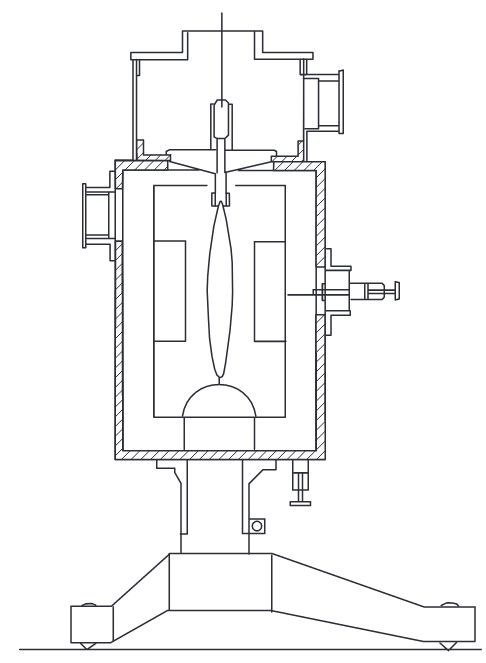
\includegraphics[width=0.35\textwidth]{content/background/figures/wulf_schema.png}
            }
        \hfill
         \subfloat[
            Ionizaiton rate from Victor Hess (left) and Werner
            Kolhörster (right)
         ]{
            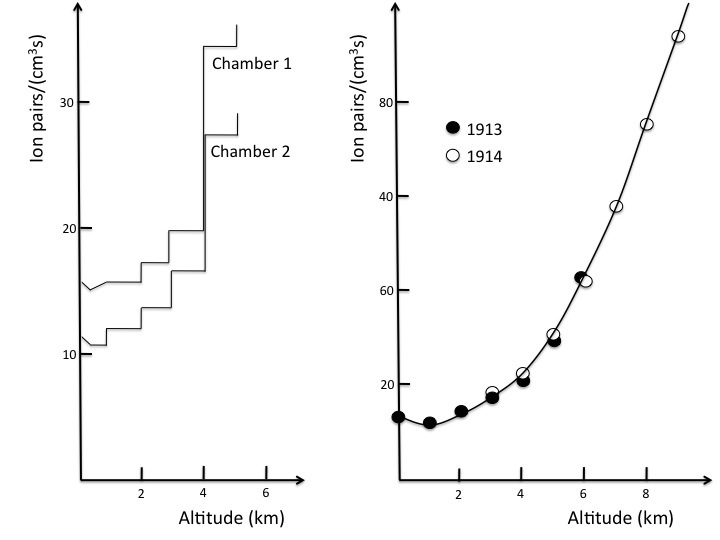
\includegraphics[width=0.6\textwidth]{content/background/figures/HessKol.jpg}
            }
        \caption{Wulf's apparatus and the ballon experimental results}
       \label{fig:xxx}
\end{figure}


However, the experiment of measuring the affect of altitude
variation with a tiny altitude scale comparing to the Earth's
atmosphere would not enough to consolidate the theory.
In the same year, the ballon with a similar instrument has
been released up to 1.3 kilometers by Karl Bergwitz to put 
more weight on the first experiment. They found that the 
ionization has increased by a quater comparing to ground level 
(\cite{de2014atmospheric}).
Three years later, suicidal investigation was conducted by 
an Australian gentleman who brought the detector and himself
to fly with the balloon.
His name is Victor Hess, people might have no doubt why this
name went so famous because he risk his life with the experiment 
and he was flying over 5 kilometers above the ground (\cite{hess1912beobachtungen}).
Definitely, the result is strongly significant and impactful
to the astrophysical research community. Risking life  
In 1914, Werner Kolhörster repeated the balloon experiment 
with higher altitude which around 9 kilometers from the 
sea level and the ionizaiton rate still does increase when 
the ballon flown higher. This emphasize that the source of 
those ionizing ray came from Earth's upper atmosphere
or the outer space.

\begin{figure}[h!]
    \centering
        \subfloat[Main  points  where  CR  intensities  were  measured  during  eight Compton expeditions in 1932]{
            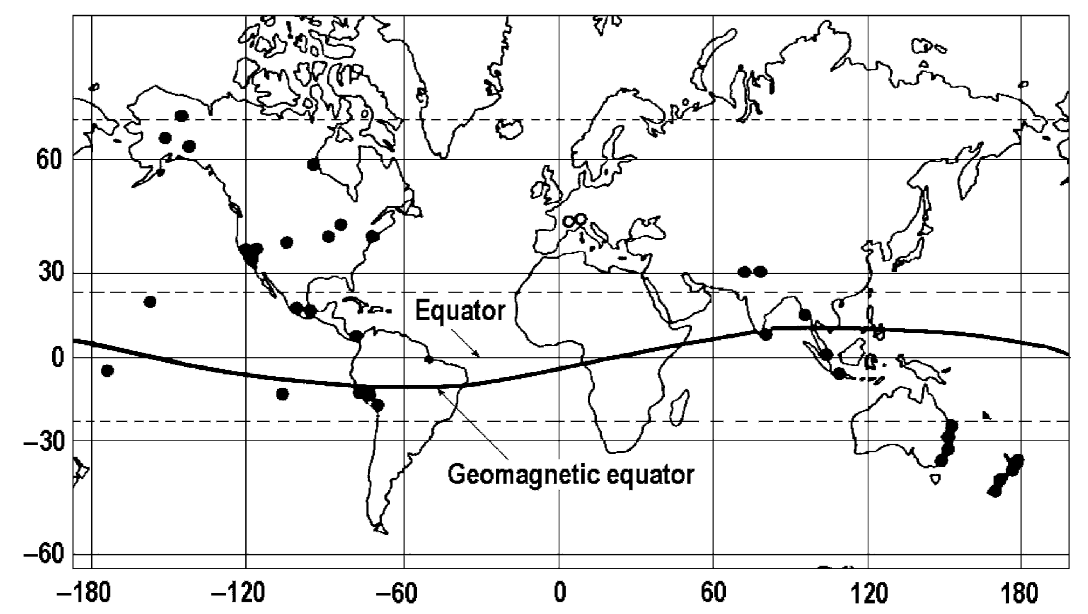
\includegraphics[width=0.62\textwidth]{content/background/figures/clay_geographical.png}
            }
        \hfill
         \subfloat[
            The Pb-shielded ionization chamber, 
            organized by Compton (\cite{text_cr_geomagnetic_effect})    
         ]{
            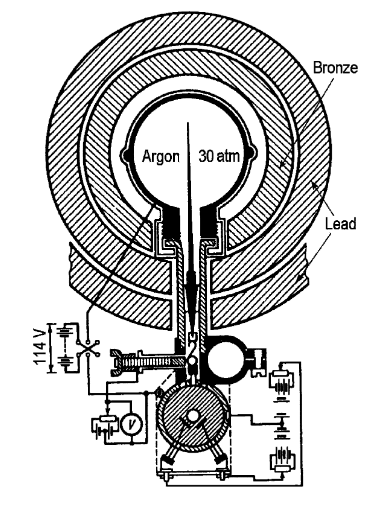
\includegraphics[width=0.32\textwidth]{content/background/figures/compton_pb_shield.png}
            }
        \caption{Clay Experiment of geographical variation}
       \label{fig:clay_cr_ship}
\end{figure}

Not only the altitude variable that related to the 
intensity of the CRs, but the geographic location of the 
obvervation also does affect to the measurement.
The first experiment has done done John Clay who
sailed the ship across the ocean from Holland to Java
(\cite{Clay1927,Clay1928}). The geographical locations 
that used to measure the CR intensities and the 
apparatus schematicical draft is shown in Figure
\ref{fig:clay_cr_ship}. The result shows that
the further from equator, the higher CR intensity.
Another exploration for the geographic variation was 
done by John Compton in the following five years.
He basically sailed the ship from the Sydney (northern hemisphere)
to Vancouver (the southern hemisphere) for various season
during 1936 to 1937 back and forth (\cite{compton1937cosmic}).
The Figure \ref{fig:comptonship} demonstrates the 
latitude variation and the seasonality effects of the 
multiple trips from the experiment.

\begin{figure}[h!]
    \centering
    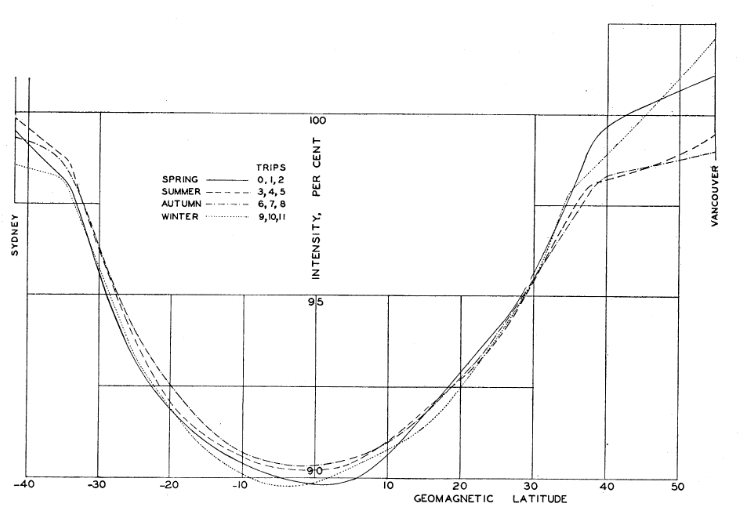
\includegraphics[width=\textwidth]{content/background/figures/compton_sail_1937.png}
    \caption{Latitude variation for various seasons (\cite{compton1937cosmic})}
    \label{fig:comptonship}
\end{figure}
	
The first interpretation study from the discovery has been
done by Carl Störmer. The explaination of the CR's altitude variation
came from the trajectory of CR particles due to geomagnetic field
(\cite{stormer1934critical}). In that period, the topic of 
geomagnetic field and the effects of CRs was quite famous.
Another impactful study of the CRs trajectory and the relevant
of Earth's magnetic field was conducted by Bruno Rossi
for predicting an asymmetry of the East-West distribution
of CR spectrum because the primary CRs does have a positive or
negative charge then the cyclic moving direction of the 
particle was induced by Lorentz force where the direction of 
the Earth's magnetic field could be identified to determine the
direction of the charged particles (\cite{rossi1941cosmic}).

The ground based detector is a great option for 
detecting the CRs where it include primary and secondary CRs.
However, investigating the primary CRs is a challenging topic
for ground based detector especially for low energy particles.
Another interesting option to inspect the asymmetry of 
East-West could be done by using space based detector 
that orbiting around the Earth's at some radius in the
higher altitude and definitely it would face a lower 
atmospheric density which consider to be an interesting 
choice to study the CRs with a lower effects of atmospheric
interaction. In 2008, \textit{Fermi} Large Area Telescope (LAT)
has been launched to observed $\gamma$-ray and
lightweight lepton particles which basically are electron
and position. The East-West effects from geomagnetic
induction was also emphasized by \textit{Fermi}-LAT.


\subsection{Physical properties}
CRs are high energy particles that propagating through
the space. The momentum of the particles came from
various acceleration mechanism base on where it from 
such as supernovae, active galactic nuclei, quasars 
and gamma-ray bursts. The composition of CRs consists of
90\% protons, 8\% alphas and other nuclei of heavier
elements (\cite{CRComposition2017}). Experimentally,
many observations indicate that the spectrum of CRs 
for all particles and individually does follow the 
power law in rigidity (momentum per charge) with a specific spectral index depends on 
their energy range. Theoretically, the observed spectrum
with a broad energy range would represented the superposition
of arrival CRs with a diverse producers where each producer
has their own specific character which is spectral index.
By the end of the day, it is barely possible to distinguish
the origin of CR particles one by one. Then it is more 
plausible to provenance the origin of CR particles in the 
macroscale rather than inspecting in the microscale.




\begin{figure}[h!]
    \centering
    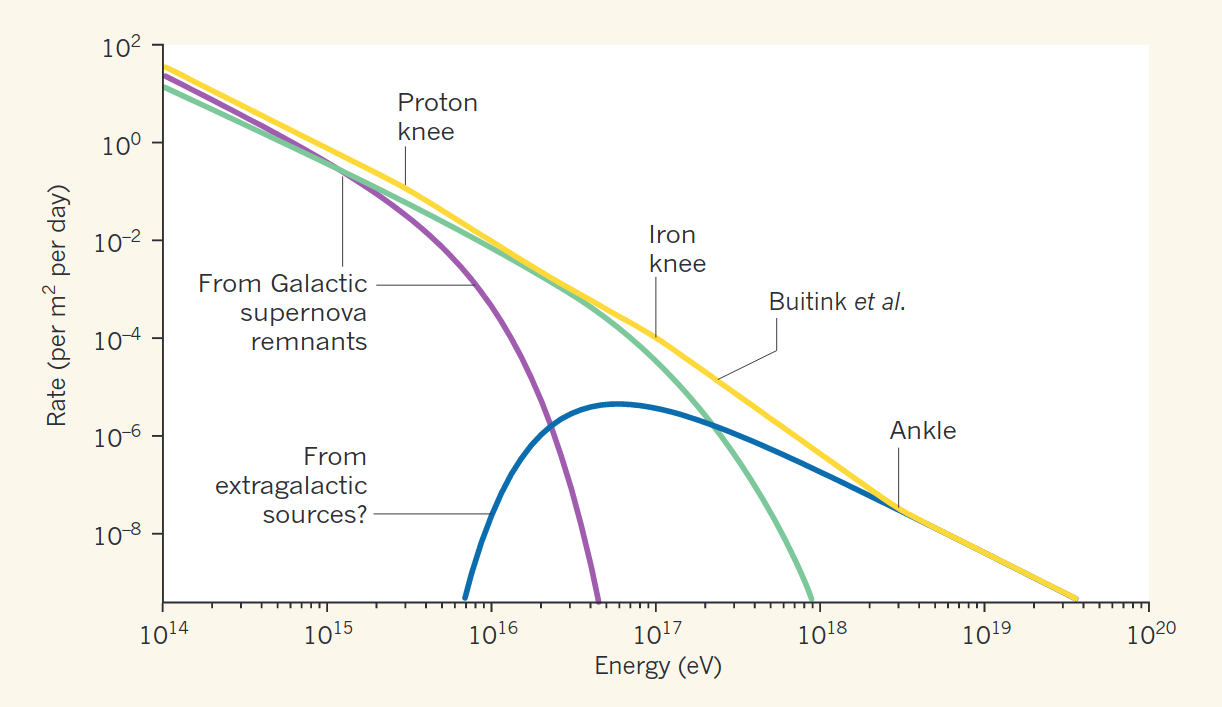
\includegraphics[width=\textwidth]{content/background/figures/andrew_superposition.png}
    \caption{Superposition of CR spectrum (\cite{taylor2016_crspectrumsuperposition})}
    \label{fig:cr_superposition}
\end{figure}

As mentioned in an early paragraph, each souce of CR does reflect their
own specific spectral index in the arrival CR spectrum.
In order to validate the theoritical assumption, putting 
the simulation or calculation of each sources and check
with the real data does compliment experimental observations.
The superposition of various sources that yield a 
discontinuity of the spectral indices has been exploided
in some energy ranges. Two well known breaking points 
are knee and ankle where it located in the energy order 
around $10^{15}$ eV and $10^{18}$ eV sequentially.
Approximately, the rate to find one particle at knee
is around one particle per square meter per year and 
the possibility that the apparatus could detect the particle
in energy at ankle point is roughly one particle per 
kilometer per year. Figure \ref{fig:cr_superposition} illustrate
the concept of superposition from various sources and 
yield the arrival CR spectrum with a breaking spectral indices. 

Not only the below ankle energy that has an interesting
properties, but the CR that has energy beyond the ankle energy
also has an identical properties. It knowns as "ultra-high
energy cosmic rays" (UHECR). One interesting point is that it 
does not that far from ankle in term of rigidity magnitude
which higher around 1 or 2 order of magnitude. The widely known 
explaination why it could not go so far is the
Greisen–Zatsepin–Kuzmin limit (GZK limit).
The theory provides the description why it the UHECR
could not propagte though the space but please note that
some sources still could produce such a UHECR but the main
issue here it the space does not empty. It contains some 
intermediate matter or dust and the microwave background radiation
which it is believed that it came from the residue of the 
Big Bang or some greate explosion or expansion of the space that 
human never saw it (at least in the human lifetime).
The main calculation of the CR kinetic energy limit from GZK 
was considered only proton particles and the main interaction
that makes it stop is basically from the interaction with 
microwave background radiation that almost perfectly
isotropically progating in the space with an order of 
traveling proton around hundred light years in the space
(\cite{gzk_cr_limit}). The way of this kind of intereaction 
not only does slow down the CR proton by producing 
neutral pion where it mostly decay into a pair of $\gamma$-rays
but it could also yield a neutron with 
a charged pion. Hence, it is also answer why we could 
see such a high energy neutron that does not only 
produced in the sky (shower effects) albeit it does not
has any charge to be accelerated in the famouse 
acceleration mechanism such as shock acceleration.

The types of CRs could be divided into two kinds based on
how they was produced which are
\begin{enumerate}
    \item \textbf{Primary cosmic rays}: they mostly be produced from the
    Solar system, somewhere in the Milky ways, extragalactic sources
    and many more. When they interact with the Earth's atmosphere,
    with the hadronic interaction with the air molecules,
    they produce the secondary CR particles.
    \item \textbf{Secondary cosmic rays}: as mentioned in collapsing of the  
    primary CRs, secondary CRs consists of many particles
    from lightweight leptons to medium weight leptons and 
    from mesons to hadron particles as well. The interaction
    of the proton with the atmospheric molecule looks simple 
    but the precise calculation from derivation is extremely complicate 
    since there are endless possibility of the (Feynman) path that 
    also produce another products with a certain probability.
    By the end of the day, we definitely got a few certains 
    of particles from their likelihood of the occurence from 
    the collision which mainly are electrons, positions, muons,
    pions and photons as demonstrates in Figure \ref{fig:cr_shower}.
\end{enumerate}

\begin{figure}[h!]
    \centering
    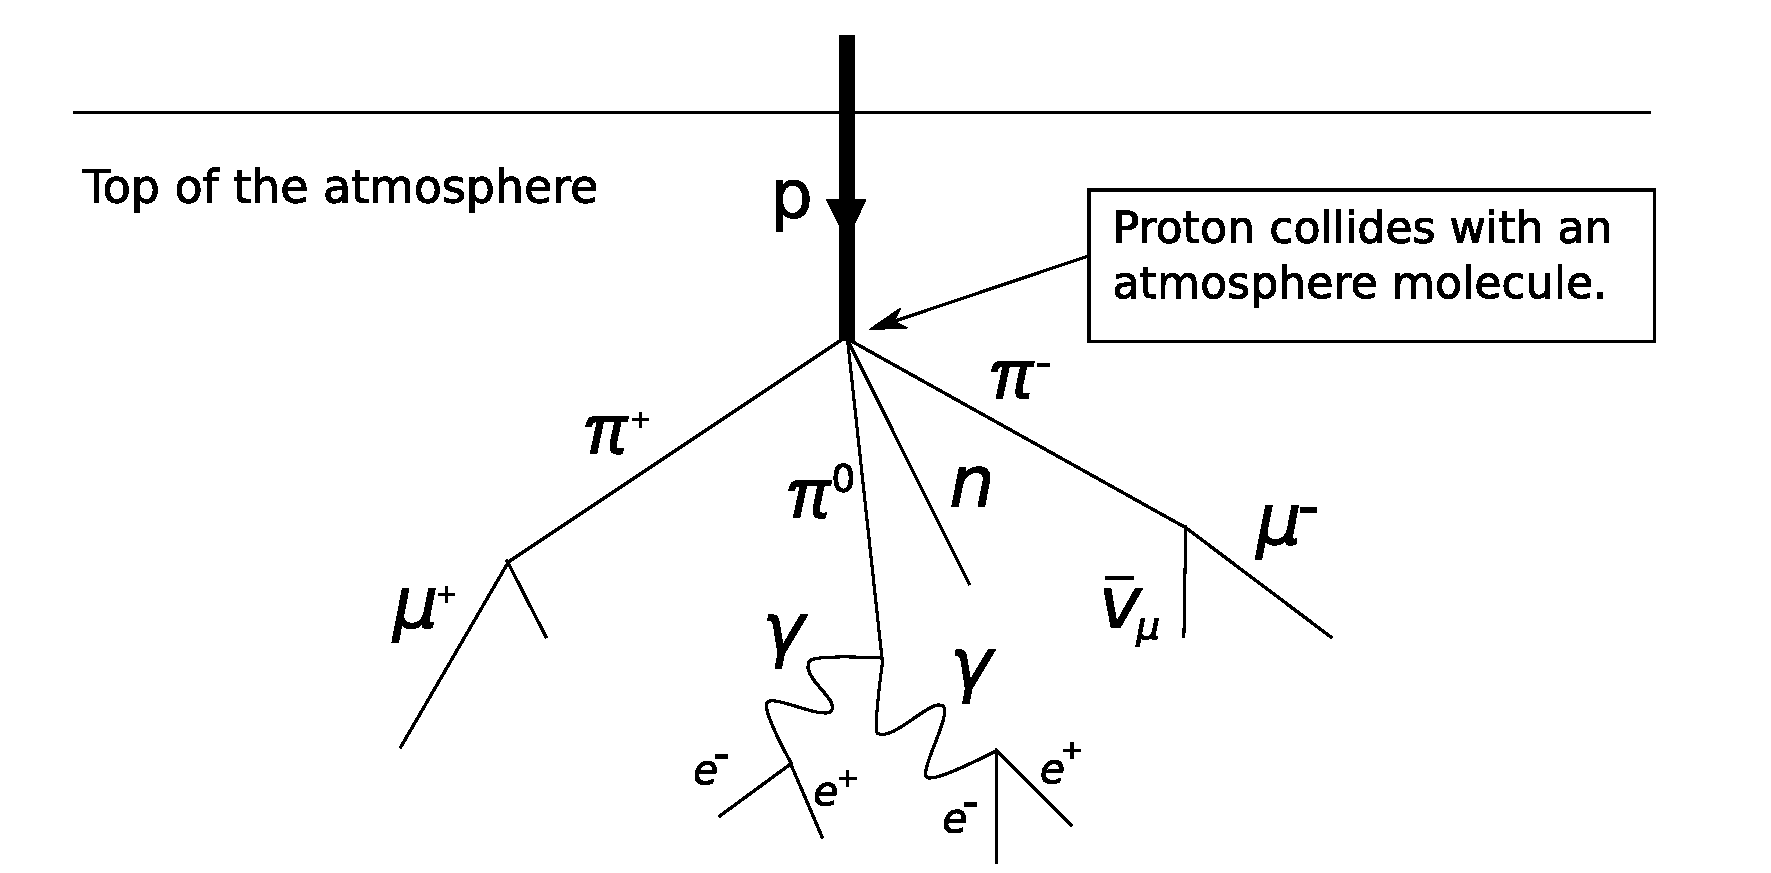
\includegraphics[width=\textwidth]{content/background/figures/Atmospheric_Collision.pdf}
    \caption{Cosmic rays shower from collision of primary CR with the atmospheric molecule
    }
    % 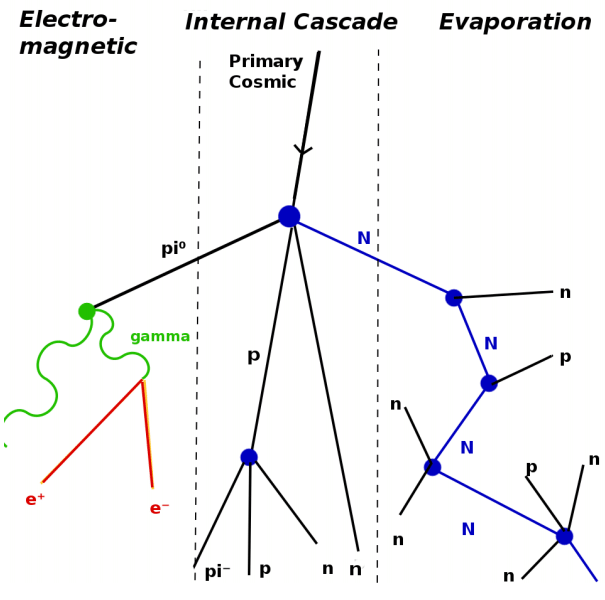
\includegraphics[width=0.7\textwidth]{content/background/figures/cr_shower2.png}
    % \caption{Cosmic rays shower from collision of primary CR with the atmospheric molecule.
    % Image taken from \cite{cr_shower_img}
    % }
    \label{fig:cr_shower}
\end{figure}


\subsection{$\gamma$-ray production}

The production of $\gamma$-ray particles happens all the 
time. It is mandatory to understand how a photon could 
gain a very high momentum from the nature. The procedure 
to acquire all those kinetic energy is quite different from how
a charged particle obtains their momentum because a 
charged particle could earn their kinetic energy during 
 their trip of propagating through the space with a 
Lorentzian force. The $\gamma$-rays mostly have only one 
chance to pick their kinetic energy and it happens when it 
was produced bacause it is barely interact with any other 
particles in the space especially high energy $\gamma$-ray.
The scenarios that makes photon hold a high energy are 
listed in the following bullets.

\subsubsection{Mechanism of $\gamma$-ray producing}

\begin{itemize}
    \item \textbf{Decaying of unstable matter}:
    Radioactive decay is one of the most well known
    phenomena for the $\gamma$-decay mode. One example 
    of the heavy ion decay is the cobalt-60. It decays 
    into excited state of nickle as

    \ch{27^{60}Co -> 28^{60}Ni^{*} + e- + $\bar{\nu}$ + $\gamma$},

    then the excited nickle decay another $\gamma$-ray
    to make it to the stable state

    \ch{28^{60}Ni^{*} -> 28^{60}Ni + $\gamma$ }.

    The famous decay of a lower level from a small 
    nuclei that consists of two quarks called "meson".
    To be more precise, it is known as the pion decay.
    The path diagram is demonstrated in Figure \ref{fig:neutral_pion_decay}
    where the neutral pion from the collision process that
    interact via Yukuwa's interaction. The neutral pion itself
    does not stable then it would have a short amount of lifetime 
    before it dominately decays into two high energy photons.
    \begin{figure}[h!]
        \centering
        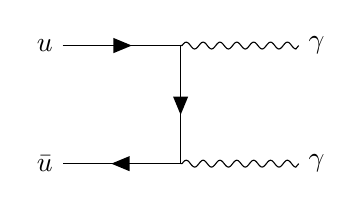
\begin{tikzpicture}
    \begin{feynman}
    \vertex (a);
    \vertex [below= of a] (b);
    \vertex [left= of a] (p1) {\(u\)};
    \vertex [left= of b] (p2) {\(\bar{u}\)};
    \vertex [right= of a] (q1) {\(\gamma\)};
    \vertex [right= of b] (q2) {\(\gamma\)};
    
        \diagram* {
            (p1) -- [fermion] (a) ,
            (a) -- [fermion] (b),
            (b) -- [fermion] (p2) ,
            (a) -- [photon] (q1),
            (b) -- [photon] (q2),
        };
    \end{feynman}
\end{tikzpicture}
% \begin{tikzpicture}
%     \begin{feynman}
%     \vertex (a);
%     \vertex [below= of a] (b);
%     \vertex [left= of a] (p1) {\(d\)};
%     \vertex [left= of b] (p2) {\(\bar{d}\)};
%     \vertex [right= of a] (q1) {\(\gamma\)};
%     \vertex [right= of b] (q2) {\(\gamma\)};
    
%         \diagram* {
%             (p1) -- [fermion] (a) ,
%             (a) -- [fermion] (b),
%             (b) -- [fermion] (p2) ,
%             (a) -- [photon] (q1),
%             (b) -- [photon] (q2),
%         };
%     \end{feynman}
% \end{tikzpicture}

% \begin{tikzpicture}
%     \begin{feynman}
%         \vertex (a);
%         \vertex [above right= of a] (b);
%         \vertex [below right= of a] (c);
%         \vertex [left= of a] (p1) {\(\pi^0\)};
%         \vertex [right= of b] (q1) {\(\gamma\)};
%         \vertex [right= of c] (q2) {\(\gamma\)};

%         \diagram* {
%             (p1) [particle] -- [scalar] (a),
%             (a) -- (b),
%             (a) -- (c),
%             (b) -- (c),
%             (b) -- [photon] (q1),
%             (c) -- [photon] (q2),
%         };
%     \end{feynman}
% \end{tikzpicture}
        \caption{Feynman's diagram of neutral pion decays into two $\gamma$-rays}
        \label{fig:neutral_pion_decay}
    \end{figure}
    Definitely, neutral pion also could yield one $\gamma$-ray
    and a pair of lightweight leptons, a couple 
    pair of lightweight leptons or even just a pair 
    of lightweight leptons and much more as long as it 
    conserve the momentum, energy and the quantum numbers.
    The main reason why the majority of their decaying process
    does yield only photons because the scattering amplitude
    as the Figure \ref{fig:neutral_pion_decay} does hold a branching
    ratio around 0.98823 and the rest of them is 
    smaller than 1\%. Another interesting property of this 
    decay mode is the momentum vector of their pair $\gamma$-ray
    hold an opposite direction with the same amplitude in the 
    reference frame.

    \item \textbf{electron–positron annihilation}:
    In the universe, there are some probability of the electron and 
    position was forced to face each other by some chance from
    the electromagnetic force or randomly found each other.
    The intereaction when they facing each other dominate by 
    electromagnetic interaction and definitely require a photon
    as a mediator to allow them talk to each other in quantum 
    electro dynamics point of view. Definitely, there is a change 
    when those pair of leptons decide to annihilate into high energy photons
    without runing any physical laws. Nevertheless, other kind of
    a pair of leptons like muon technically could deforms into two
    photons with much higher energy because their rest mass is higher.
    Surely, a pair of Tau is also allow to produces a pair of photons.
    However, the lifetime of those medium-weight and heavy-weight leptons
    could not last that long to survive in practical. The simplest 
    Feynman's path of annihilation of leptons into a pair photons 
    is illustrated in Figure \ref{fig:lepton_annihilation} from light 
    to heavy leptons sequentially.

    \begin{figure}[h!]
        \centering
            \subfloat[
                Lightweight leptons
            ]{
                \begin{tikzpicture}
\begin{feynman}
\vertex (a);
\vertex [below= of a] (b);
\vertex [above left= of a] (p1) {\(e^{-}\)};
\vertex [below left= of b] (p2) {\(e^{+}\)};
\vertex [above right= of a] (q1) {\(\gamma_1\)};
\vertex [below right= of b] (q2) {\(\gamma_2\)};

    \diagram* {
        (p1) -- [fermion] (a) ,
        (a) -- [fermion] (b),
        (b) -- [fermion] (p2) ,
        (a) -- [photon] (q1),
        (b) -- [photon] (q2),
    };
\end{feynman}
\end{tikzpicture}
            }
            \hfill
            \subfloat[Mediumweight leptons]{
                \begin{tikzpicture}
    \begin{feynman}
    \vertex (a);
    \vertex [below= of a] (b);
    \vertex [above left= of a] (p1) {\(\mu^{-}\)};
    \vertex [below left= of b] (p2) {\(\mu^{+}\)};
    \vertex [above right= of a] (q1) {\(\gamma_1\)};
    \vertex [below right= of b] (q2) {\(\gamma_2\)};
    
        \diagram* {
            (p1) -- [fermion] (a) ,
            (a) -- [fermion] (b),
            (b) -- [fermion] (p2) ,
            (a) -- [photon] (q1),
            (b) -- [photon] (q2),
        };
    \end{feynman}
    \end{tikzpicture}
            }
            \hfill
            \subfloat[
                Heavyweight leptons
             ]{
                \begin{tikzpicture}
    \begin{feynman}
    \vertex (a);
    \vertex [below= of a] (b);
    \vertex [above left= of a] (p1) {\(\tau^{-}\)};
    \vertex [below left= of b] (p2) {\(\tau^{+}\)};
    \vertex [above right= of a] (q1) {\(\gamma_1\)};
    \vertex [below right= of b] (q2) {\(\gamma_2\)};
    
        \diagram* {
            (p1) -- [fermion] (a) ,
            (a) -- [fermion] (b),
            (b) -- [fermion] (p2) ,
            (a) -- [photon] (q1),
            (b) -- [photon] (q2),
        };
    \end{feynman}
    \end{tikzpicture}
            }
            \caption{Major lepton annihilation path diagram}
           \label{fig:lepton_annihilation}
    \end{figure}

    \item \textbf{Synchrotron radiation\& Bremsstrahlung radiation}:
    The phenomena of turning momentum direction of charged particle
    or accelerate into another direction shares a similar
    description. Conservation of momentum has come into place when 
    considering the bending charged particle that would emit the
    photon. Regarding the incoming direction of a charged particle 
    and then turning it direction by $\pi/2$ radians. The question
    that comes into mild is where does those initial momentum in an 
    incoming direction does since the momentum is conserved along 
    the cartesian direction, not only the magnitude. Now the clue is 
    here, they have to emit the photon to converse the momentum of 
    the system.
    
    Let walk through the first example called
    synchrotron radiation. Keeping some charged particle circulating 
    around the donut-like apparatus have some cost to pay to make 
    them stay without escaping the tunnel. Unquestionably, draging
    some moving particle circulating around some point requires a
    centripedal force. In this case, applying electromagnetic force
    without toucing it would yield a radiation called synchrotron emission.

    The second mechanism is Bremsstrahlung, where a charged particle 
    or typically an electron moving path close to some opposite charged 
    particle or typically a proton. The explaination from Coulomb's law
    would cover this scheme for the definition that the force is 
    inverse proportional to the distance between two charges. Then 
    moving pass by an opposite charged particle does induced the electron
    bending and emit the photon because the explained reason from the 
    previous paragraph. This mechanism happens when an CR electrons 
    moving through the matter of Sun's chronosphere and interact with 
    a positive charged and produce some high energy photon but usually 
    it produce in the X-ray energy range.


\end{itemize}



% decel & ac cel
\subsubsection{Mechanism of $\gamma$-ray gaining momentum}

Even though, $\gamma$-ray usually does not prefer
to talk to another fundamental particles because
scattering amplitude of their interaction is pretty 
low. Nonetheless, there are some scenarios that $\gamma$ could 
gain more kinetic energy and losing their kinetic energy 
when they traveling in the universe.

\begin{itemize}
    \item \textbf{Inverse Compton scattering}
    The scattering of a photon (massless particle) with an electron 
    (massive particle) could occur during their trip. Equation \ref{eq:inv_compton} 
    demonstrate the symbolic relation of the scattering with the 
    electromagnetic interaction and yield the same particles as an 
    incoming particles.

    \begin{equation}
        e^-\gamma \rightarrow e^-\gamma
        \label{eq:inv_compton}
    \end{equation}

    Interaction between an electron and a photon could 
    make them converting the momentum via the scattering
    processs. Since the system momentum has to be conserved,
    then there will be one losing momentum and another one gaining 
    momentum or kinetic energy. Suppose one photon is traveling 
    and hit electron or a charged particle, it could transfer the 
    kinetic energy to the particle and their wavelength will be 
    longer. In another word, it is lossing the kinetic energy.
    On the other hand, this scenario could happen in the opposite way.
    There is situation when a high energy electron interacting with 
    the photon and turn over it kinetic energy to the photon. After that,
    a photon could gain more kinetic energy during their trip. 
    The latter scenario is called "Inverse Compton Scattering".
    The most likelihood choice of interaction of the scheme could be 
    represented in Feynman's path as in Figure \ref{fig:compton_feynman}.

    \begin{figure}[h!]
        \centering
            \subfloat[First branch]{
                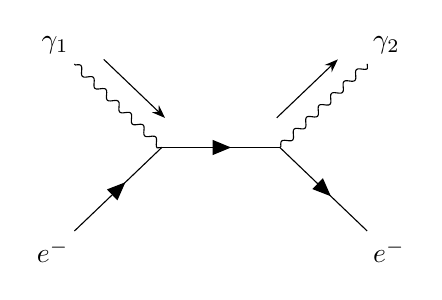
\begin{tikzpicture}
    \begin{feynman}
    \vertex (a);
    \vertex [right= of a] (b);
    \vertex [below left= of a] (p1) {\(e^{-}\)};
    \vertex [above left= of a] (q1) {\(\gamma_1\)};
    \vertex [below right= of b] (p2) {\(e^{-}\)};
    \vertex [above right= of b] (q2) {\(\gamma_2\)};
  
      \diagram* {
        (a) -- [fermion, edge label'=\(\)] (b) ,
        (q1) -- [photon, momentum] (a) ,
        (p1) -- [fermion] (a),
        (b) -- [photon, momentum] (q2),
        (b) -- [fermion] (p2),
      };
      \vertex [below= 0.5em of a] {\(\)};
      \vertex [below= 0.5em of b] {\(\)};
    \end{feynman}
  \end{tikzpicture}
                }
            \hfill
             \subfloat[
                Second branch
             ]{
                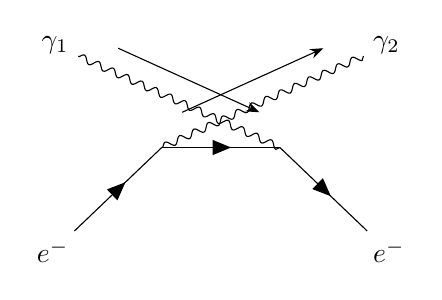
\begin{tikzpicture}
    \begin{feynman}
    \vertex (a);
    \vertex [right= of a] (b);
    \vertex [below left= of a] (p1) {\(e^{-}\)};
    \vertex [above left= of a] (q1) {\(\gamma_1\)};
    \vertex [below right= of b] (p2) {\(e^{-}\)};
    \vertex [above right= of b] (q2) {\(\gamma_2\)};
  
      \diagram* {
        (a) -- [fermion, edge label'=\(\)] (b) ,
        (q1) -- [photon, momentum] (b) ,
        (p1) -- [fermion] (a),
        (a) -- [photon, momentum] (q2),
        (b) -- [fermion] (p2),
      };
      \vertex [below= 0.5em of a] {\(\)};
      \vertex [below= 0.5em of b] {\(\)};
    \end{feynman}
  \end{tikzpicture}

                }
            \caption{Trivial Feynman's path of (Inverse) Compton scattering}
           \label{fig:compton_feynman}
    \end{figure}
\end{itemize}




\subsubsection{$\gamma$-ray production plants}



\begin{itemize}
    \item \textbf{Supernova ramnants (SNRs) and molecular cloud}: 
    The supernova explosion is a huge expansion from that approximately
    expanding as a spherical shell that sweep the inter stellar medium (ISM)
    and decelerate at some radius after the enlargement. The kinetic 
    energy that transfer from the momentum in the radial axis was 
    modeled and belived to be the kinetic energy of the cosmic ray particles.
    There are three major processes that involves in this phenomenon which 
    are nuclear pion production, nonthermal electron bremsstrahlung, and Compton scattering
    (\cite{cr_from_snr_2013}). Last but not least, the shock acceleration
    could play an important role for this phenomenon.

    \item \textbf{Diffused $\gamma$-ray emission from galactic plane}:
    One of the bright source that does not locate too far from our teritory
    is the galactic plane. The first reasonable explaination is the 
    distance of the productive objects does not far from Earth comparing 
    to other extragalactic sources. In addition, there are many interesting 
    CR sources in our galaxy. It might be pulsar, some flare of the 
    event of an explosion and so on. The plot that shows the brightness
    of the galactic plane comparing to the outer space is shown in 
    Figure \ref{fig:gamma_galac_plane}.

    \begin{figure}[h!]
        \centering
        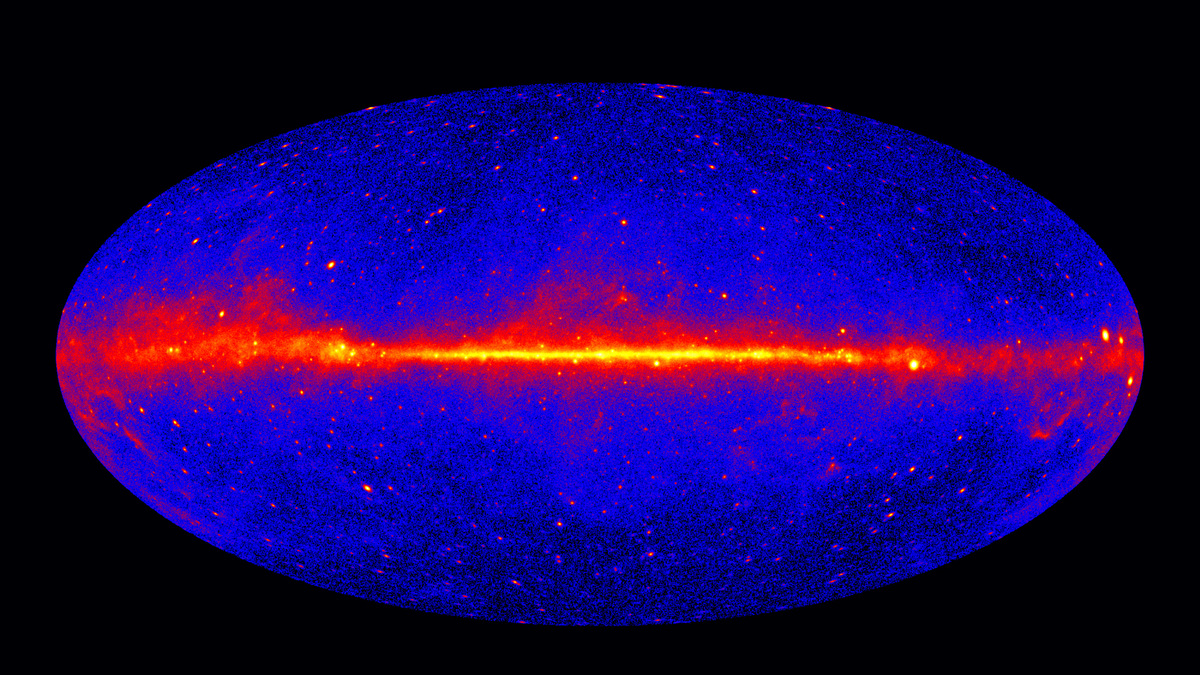
\includegraphics[width=\textwidth]{content/background/figures/Fermi_5_years.jpg}
        \caption{Intensity of $\gamma$-ray $>$ 1 GeV in galactic coordinate (Image credit: NASA/DOE/\textit{Fermi} LAT Collaboration)}
        \label{fig:gamma_galac_plane}
    \end{figure}

    \item \textbf{Pulsar and Active Galactic Nucleus (AGN)}: 
    Another source of the brightness in Figure \ref{fig:gamma_galac_plane}
    is the bright dots with a different solid angle width in the sky.
    The majority of those spots consists of $\gamma$-ray from 
    pulsar's periodic emission and AGN or extremely luminous AGN
    namely "Quasar". The cycle of the lighthouse effects from pulsar 
    is very robust as in the scale of atomic clock. Both of them 
    has a very high magnetic field strength. Emissive photons from 
    those sources would be a very high energy due to the accelation 
    of a charged particle near magnetic poles or the outer.


    \item \textbf{Earth's limb $\gamma$-ray production}:
    The closest $\gamma$-ray source is our Earth's atmosphere.
    To be more precise, the Earth's upper atmosphere is super bright 
    in $\gamma$-ray exposure. The main reason that cause the shining 
    of Earth's limb does came from the collision of the CR's massive
    particle such as protons and alphas. The interaction of those high 
    energy CR massive particles yield many more particles and main 
    contribution of the $\gamma$-ray dazzling came from the neutral pion
    decay which is the product from the collision process.

\end{itemize}



%%%%%%%%%%%%%%%%%%%%%%%%%%%%%%%%
%         Fermi-LAT
%%%%%%%%%%%%%%%%%%%%%%%%%%%%%%%%
\section{\textit{Fermi} Large Area Telescope (LAT)}
One of the famous space telescope that does see the sky in the 
visible wavelength is \textit{Fermi} Large Area Telescope (LAT).
Formerly, it was called Gamma-ray Large Area Space Telescope (GLAST).
The mission of the satellite is to collect high energy photon data 
or $\gamma$-ray and it technically could detect the lightweight
lepton particles namely electron and position.
The orbiting radius is around 550 kilometers
from the sea level. It is designed for observing the full-sky in 
$\gamma$-ray region. It also attach the Gamma-ray Burst Monitor (GBM) to study gamma-ray
bursts for seeking an exotic event. The telescope was launched in 
11 June 2008 at 16:05 UTC or 21:05 Bangkok time by abroading with 
Delta II 7920-H rocket.


\subsection{Overview}

\begin{figure}[h!]
    \centering
    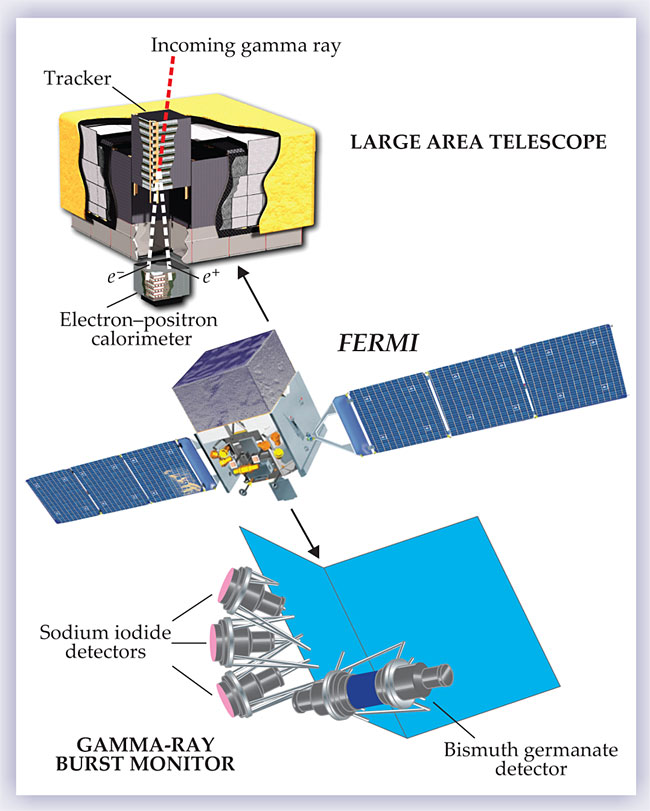
\includegraphics[width=0.6\textwidth]{content/background/figures/fermi_instrument.jpeg}
    \caption{Main components of \textit{Fermi}-LAT (Image taken from \cite{fermi_lat_instrument_first_year})}
    \label{fig:fermi_main_components}
\end{figure}
According to Figure \ref{fig:fermi_main_components},
each components of the $Fermi$ telescope was designed for a purpose since there 
is no ideal detector module that could detect kind of particles.
There are two main parts where the first part if the major component 
called Large Area Telescope (LAT) for detecting the $\gamma$
-ray and the second part is Gamma-ray Burst Monitor (GBM) for seeking 
an interesting event in the sky. In fact, both of them does detect 
the $\gamma$-ray but in the different energy scale. LAT is the main 
component where it detect the $\gamma$-ray in a few dozen of GeV 
up to a digit of TeV. For GBM part, the visible photon energy 
for them is around 8 keV to 40 MeV. The GBM consists of two 
sub components which are sodium iodide detector for low-energy photons
(8 keV to 1 MeV) and bismuth germenate detector for high-energy photons 
(0.2 MeV to 40 Mev). GBM detectors distribute around 
the telescope to be a closed circuit camera and looking for a flare 
of the $\gamma$-ray. The actual purpose of GBM is not a detector 
for collecting a high quality data but it is attached in the spacecraft 
to assist the LAT for mainly looking at an interesting events that could 
produce a huge amount of $\gamma$-rays. The content in this chapter 
will deep down into more detail of LAT in depth and would not provide 
more detail of GBM.

\subsection{Large Area Telescope (LAT)}


\begin{figure}[h!]
    \centering
    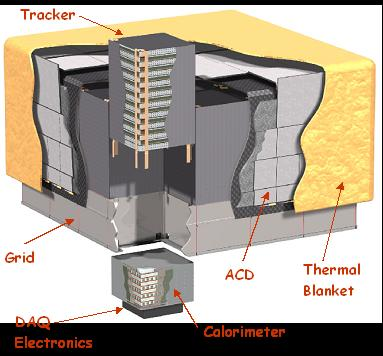
\includegraphics[width=0.6\textwidth]{content/background/figures/LATStructure.jpg}
    \caption{Instrument structure (Image taken from https://fermi.gsfc.nasa.gov)}
    \label{fig:fermi_lat_structure}
\end{figure}

LAT consists of tracker (TKR) module for tracing the incoming photon,
calorimeter (CAL) for measuring the kinetic energy after the particle 
has been passed through the tracker because a charged particle 
interact with the CAL and dissipate since it enter the module
and anti-coincidence Detector (ACD) for rejecting the background 
signal. The last part is the on-boarding data acquisition (DAQ)
module for investigating the particle's footprint and digitize
the signal.


\begin{figure}[h!]
    \centering
    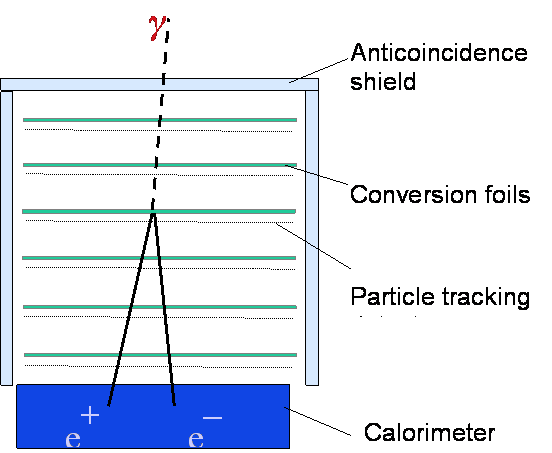
\includegraphics[width=0.6\textwidth]{content/background/figures/LAT_layers.png}
    \caption{Schematic structure of the LAT (Image taken from https://fermi.gsfc.nasa.gov)}
    \label{fig:fermi_lat_layers}
\end{figure}




\subsubsection{Tracker}
Higher energy photon or $\gamma$-ray talk to the LAT by converting the
kinetic energy into a pair of lightweight leptons or e$^{+}$e$^{-}$ pair.
The converter-tracker has 16 planes of a large atomic numbers for 
making the incident $\gamma$-ray convert into a pair of e$^{+}$e$^{-}$
as demonstrated in Figure \ref{fig:fermi_lat_layers}. After that, 
a pair of leptons would leave a footprint as an electromagnetic induction 
in particle tracker where it sensitive for the moving charge particle.

\begin{figure}[h!]
    \centering
    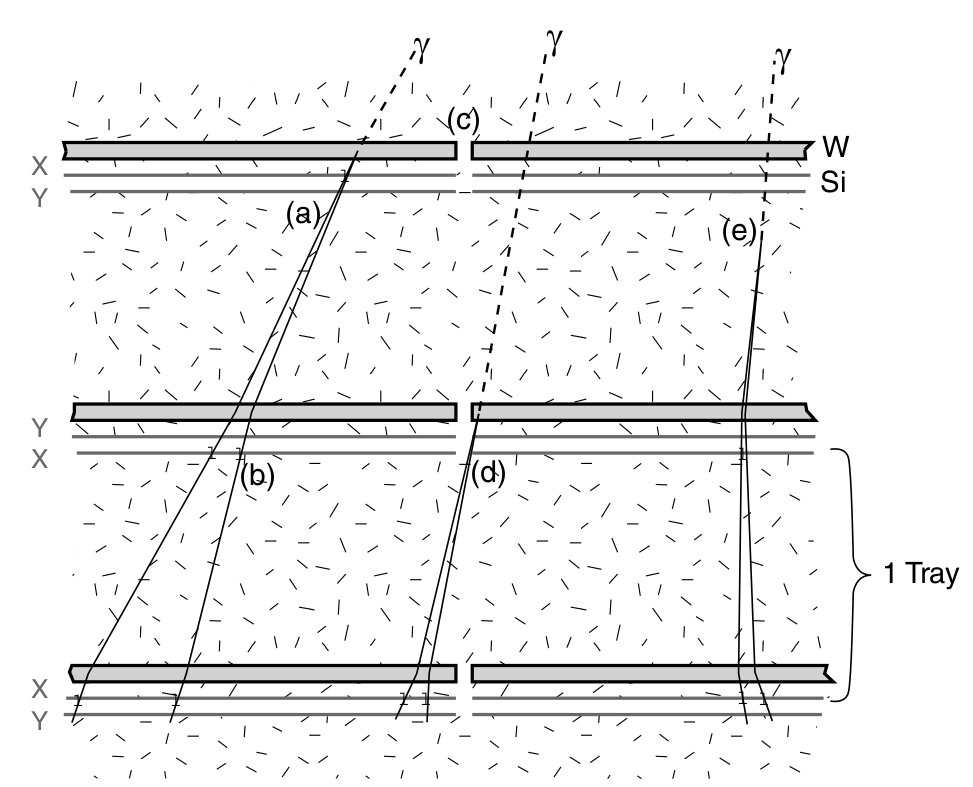
\includegraphics[width=0.6\textwidth]{content/background/figures/fermi_tracker.png}
    \caption{LAT's particle tracker (Image taken from \cite{FermiLAT})}
    \label{fig:fermi_tracker}
\end{figure}

The particle tracking is made from silicon-strip. Tracking information 
would leave the track in 2-D plane of a particle tracking. In order to
trace back and gaining data as the 3-D moving direction, 16 particle 
tracker has to be taken in account for constructing the electron 
or positron path.
Despite one layer of particle tracking could obtain 
the information about incoming leptons for x-y plane only, but techinical 
design of LAT does put a 2 layers of silicon-based tracker with a very 
narrow gap between them. This kind of design could make the LAT performing 
measurement precision in the angular resolutiom better than a single 
layer of a wide gap which affects in the point-spread function (PSF)
of the probability distribution from reconstruction direction.
According to Figure \ref{fig:fermi_tracker}, top and the bottom of
silicon trackers and the heavy-nuclei conversion layer called "Tray".
Case (a) and (b) in the figure is the ideal case where the $\gamma$-ray
hit the conversion layer and multiple footprints are recorded.
Nevertheless, there is an edge case as in (d) and (e) where the $\gamma$-ray
has a probability to skip an early layer and choose to covert in the 
secondary conversion layer and will be detected in the upcoming 
tracking layer. The major benefit of deploying multiple conversion 
layers is quite obvious for the better event gathering.


\subsubsection{Calorimeter}
Unlike particle tracker that talk to a charged particle by utilizing
the EM induction without (or barely) disturbing the particle state,
calorimeter is a starving component. It consume a lepton and produce 
electronic readout of the energy from radiation of the lepton in the
crystal scintillator. Definitely, size of this part is mainly considered 
from the radiation lengths of the electron and position particles becasue it 
has to record the shower that happen during the decaying process.
However, the radiation length highly depends on the kinetic energy 
of the particle. The LAT itself has been designed for detecting photon 
energy range between MeV to a few hundred GeV. Hence, the exposure of 
photon energy beyond TeV is probably not promising in this case.


\begin{figure}[h!]
    \centering
    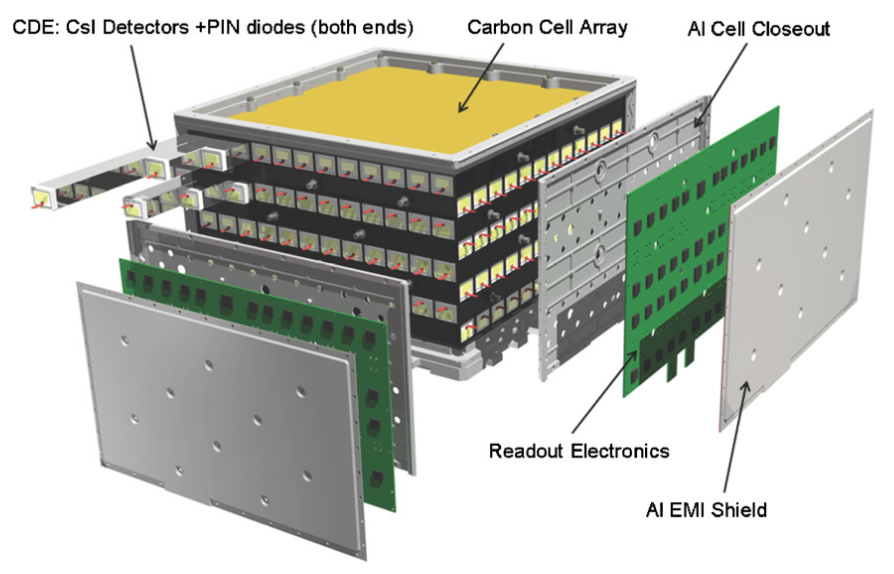
\includegraphics[width=0.8\textwidth]{content/background/figures/fermi_calorimeter.png}
    \caption{LAT's calorimeter (Image taken from \cite{FermiLAT})}
    \label{fig:fermi_calorimeter}
\end{figure}

The overview apparatus structure is illustrate in Figure \ref{fig:fermi_calorimeter}.
Each calorimeter module consists of 96 CsI(Tl) scintillator crystal size 
2.7 cm x 2.0 cm x 32.6 cm and PIN photodiodes at both ends which connect 
to the readout electronic components for translate an amount of light 
that has been sparked in the crystal to digitized signal. Each horizontal 
layer is combined from 12 crystal component and stack them 8 times by 
rotate them 90\textdegree each for boosting the angular resolution 
from the sparking lights. The carbon cell was build for supporting 
the structure of low mass particle tracker due to the properties of 
high stiffness, thermal conductivity and thermal stability.
An electron, position or $\gamma$-ray will deposit the energy in the
calorimeter as the scintillated lights via electromagnetic intereaction.
The segmented crystal also allow LAT to trace the shower
as the spatial imaging.


\subsubsection{Anti-coincidence Detector (ACD)}
The main objective of ACD is to support the charged-particle background 
rejection of the CRs. It is cover the tracker over the LAT field of 
view (FoV) for 4 side and the top part of the LAT. It consists of 
89 plastic scintillator tiles with 5 $\times$ 5 array on top and 
4 sides of 16 tiles. Each tile component contains two photomultiplier 
and wanelength shifting fibers embedded in the scintillator. The tile 
is overlapping another one in one-dimension to reduce the effect of 
the gaps between them. To be more prcise, there are two sets 
of four called scintillator ribbon for covering the top-down side 
and a pair around their center. The ACD is required to has 0.9997 efficientcy 
for detecting an incoming charged particle of FoV of the LAT. However,
the $\gamma$-ray induce the shower that calorimeter will absorb but 
there is a scenario called "backsplash effect" where the secondary 
particles in keV range from the electromagnetic shower could interact 
with the incoming photon and Compton scattering in ACD. Then it could 
create a veto signal from the recoil electron. In order to solve this issue,
the ACD with their neighborhood would take the incident candidate photon 
into account and could dramatically reduce the effect of the backsplashing.


\subsubsection{Data Acquisition System (DAQ)}


To acquire an interesting event, event selection could not be done 
on software on the ground level from the whole raw signal of subsystems because the limitation 
of the hardware in the current edge. In order to collect an event, 
raw data will be selected from filtering algorithm on board.
The hierarchical structure of data acquisition system (DAQ) was invented 
for seeking an transient event as shown in Figure \ref{fig:fermi_daq}.

\begin{figure}[h!]
    \centering
    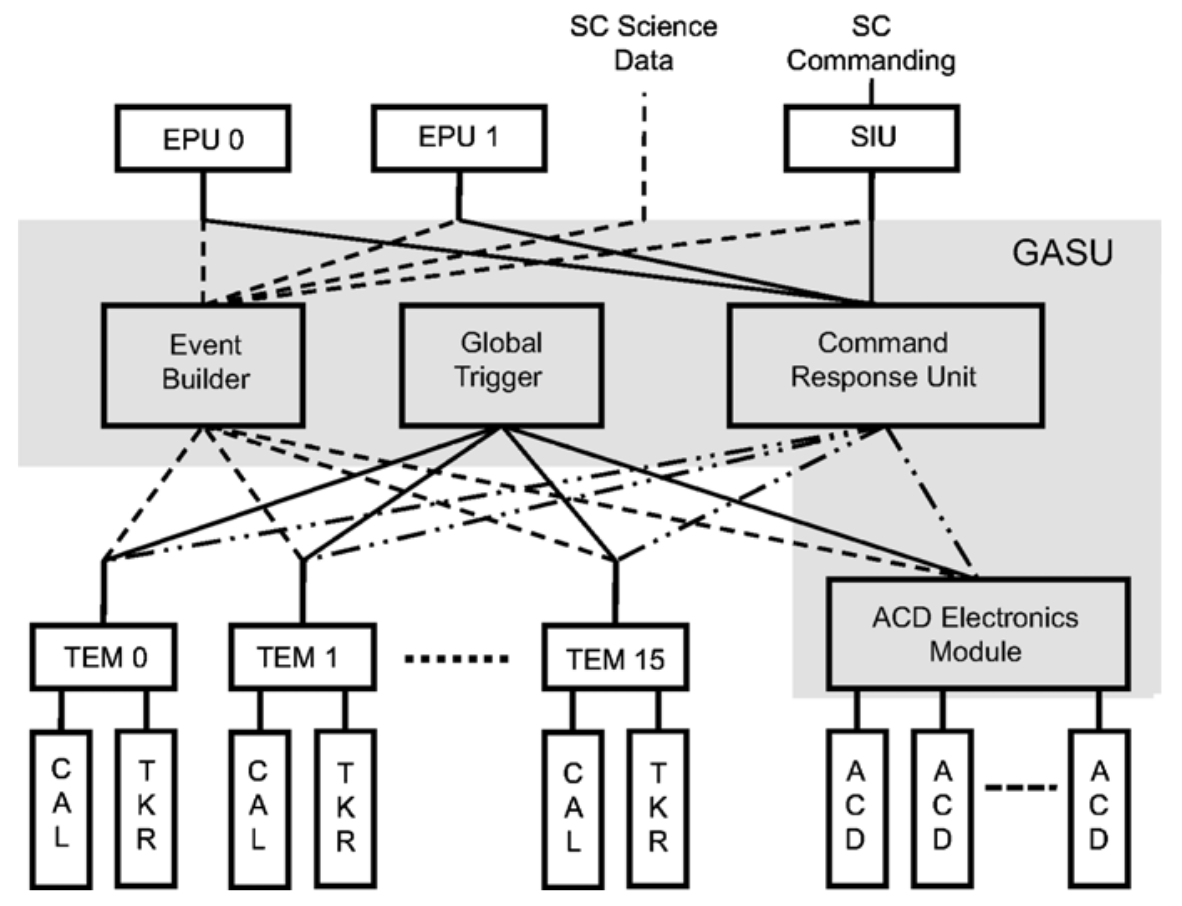
\includegraphics[width=0.6\textwidth]{content/background/figures/fermi_daq.png}
    \caption{Flow chart of LAT's data acquisition system (DAQ) (Image taken from \cite{FermiLAT})}
    \label{fig:fermi_daq}
\end{figure}

The lowest level is tower electronic modules (TEMs) to serve as an 
interface for the tracker and calorimeter. All TEMs create event 
buffering and communicates with Event Builder Module (EBM) which is a
component of Global-trigger/ACD-module/Signal distribution Unit (GASU).
Command Response Unit (CRU) was built to communicate the
software execution in DAQ system. Lastly, Event Processing Unit (EPU)
will process a selecting event from TEM and ACD Electronics Module (AEM).
Filtering an event could reduce the information flowing rate from 
a few kHz to around 400 Hz which will be sent back to the ground level.


\subsection{Event reconstruction}

In an early day, the reconstruction algorithm for tracing a photon 
is Monte Carlo (MC) simulation. Modeling the incident $\gamma$-rays 
and the background has been simulated in the orbiting-like environment 
before it launch. Meaning that background rejection property already 
embedded in the LAT since the developing process. The simulation 
could be use for the detector calibration since the simulation software 
provide an interaction physical process.

The main logic of the reconstruction is started by tracking the footprint 
in the tracker and expect the output in calorimeter cube as physical process 
would yield. After that the event classificaiton mainly consider from 
the ACD part to classify an event types.

The result from processed data on the fly is level 0 and it will pass 
down to Earth and reconstructing the photon data called level 1.
The more LAT orbiting around the Earth's, the more understanding of the 
LAT environment and it brings the software improvement for the reconstruction
algorithm to exploid the technique of pattern recognitions.
First official released is LAT data is Pass 6 and Pass 7 after has been 
released with the same level 0 data but the reconstructed event is 
more efficient than the older one by software level. The newest version 
and likely to be the final version is Pass 8. Not only the reconstruction
algorithm that has been devided but the event class is also an 
crucial concept. As mentioned earlier, the photon is clsssified into 
a specific class. There is no free lunch to think that the detector see 
the particle as a binary classificaiton. It will mix with a likelihood 
or probability to distinguish the specific kind of interesting event.
That is the main reason why \textit{Fermi}-LAT team split the event 
into multiple classes which mainly are TRANSIENT, SOURCE, ULTRACLEAN and 
ULTRACLEANVETO.

Definitely, lesser photon candidates has been selected in 
the ULTRACLEANVETO. Then there is no certain right or wrong for
picking the class from researcher point of view. The main criteria 
would be the objectives of the analysis. If the analyzer want a 
huge events and could accept some noisy event, then SOURCE or 
TRANSIENT class is suitable for the analysis and vice versa.


\subsection{Detector performance and their characteristics}

\begin{figure}[h!]
    \centering
    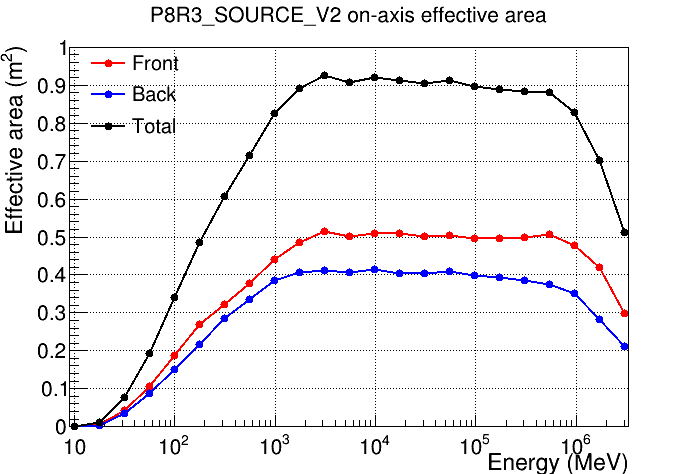
\includegraphics[width=0.7\textwidth]{content/background/figures/eff_energy.png}
    \caption{
        Effective area along the photon energy range from MeV to TeV
        (\cite{lat_p8_performance})
    }
    \label{fig:eff_energy}
\end{figure}

\textit{Fermi}-LAT has been designed for detecting $\gamma$-ray in the 
space which means that the range of energy that it could see precisely 
will starting at MeV up to TeV. The effective area in square-meters
is defined from the front and the back of the LAT's tracking layer 
by consider the upper part as a front and the bottom part belowing 
a certain layer as the back part. Since both front and back part 
components is made by the same materials and exactly same design. 
Then total effective area could be sum into a single value. 
The Figure \ref{fig:eff_energy} visualize the effectiveness of LAT 
along a given energy range. According to the plot, LAT performs 
a measurement well from GeV up to TeV scale.


Another crucial part when dealing with LAT effectiveness is the 
incidence angle ($\theta_\text{LAT}$). It highly affects to the 
number of tracking layers. The higher probability of passing more 
tracking layers would yield a better LAT's performance. Figure 
\ref{fig:eff_theta} shows relation of effective area versus 
incidence angle.


% angle dependency 
\begin{figure}[h!]
    \centering
    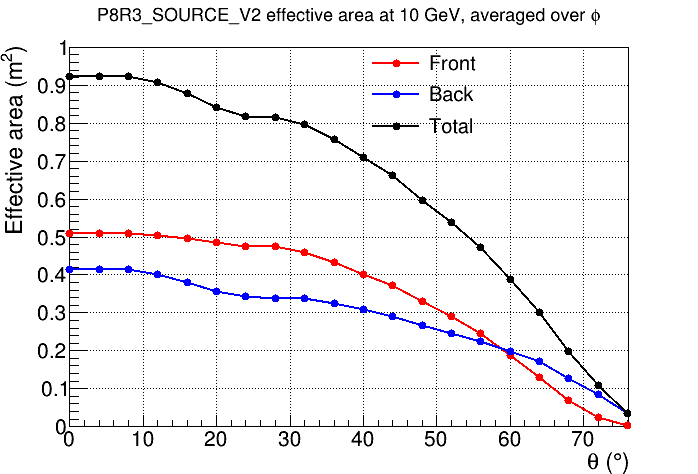
\includegraphics[width=0.7\textwidth]{content/background/figures/eff_theta.png}
    \caption{Effective area versus incidence angle (\cite{lat_p8_performance})}
    \label{fig:eff_theta}
\end{figure}

Imagine the LAT structure as a cube-like detector. Surely, the LAT 
boresight is a square where an azimuthal angle ($\phi_\text{LAT}$) of the incoming 
photon would affect a larger area that the photon could intereact 
as demonstrates in Figure \ref{fig:eff_theta}. The reason why there 
is a peak for any cycle of $\pi/2$ radian or 90\textdegree is 
the edge of the LAT would has more area to interact than the 
lateral. Another evidence for the explaination is the front effective 
area has less effects since the propagation length is narrow than 
the back.

\begin{figure}[h!]
    \centering
    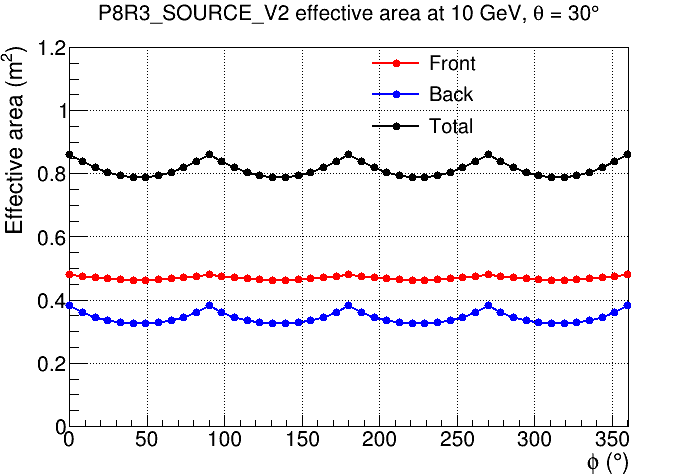
\includegraphics[width=0.7\textwidth]{content/background/figures/eff_phi.png}
    \caption{Effective area versus azimuthal angle (\cite{lat_p8_performance})}
    \label{fig:eff_phi}
\end{figure}

% event class
\begin{figure}[h!]
    \centering
    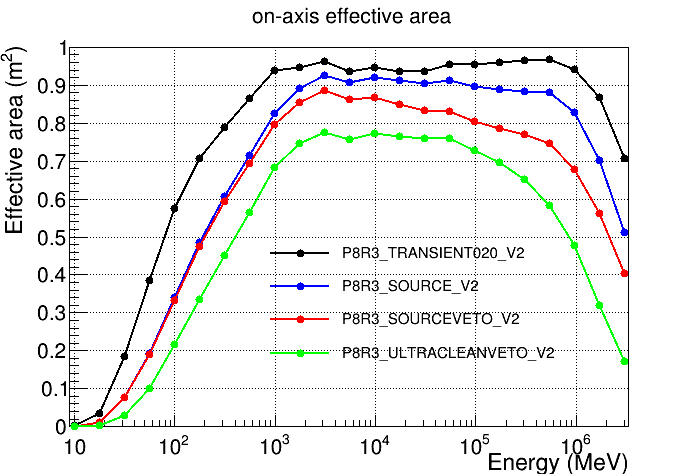
\includegraphics[width=0.7\textwidth]{content/background/figures/eff_event_class.png}
    \caption{Effective area along the energy of each event class (\cite{lat_p8_performance}))}
    \label{fig:eff_event_class}
\end{figure}


From the previous subsection, the event class is also play crucial 
role when considering the effectiveness of the reconstructed event.
Undoubtly, the cleanest class namely "ULTRACLEANVETO" would has 
the worst effective area. In opposite, TRANSIENT class would yield 
the best effective area as visualized in Figure \ref{fig:eff_event_class}.

To sum up, the effective area act for the LAT performance for seeking 
an event in the unit of square lengths. It is also behave like a function 
in the practical analysis which pragmatically allow the client to 
throw incidence angle, azimuthal angle and the energy. Then it will 
return the effective area in unit of square centi-meters in the raw 
format.

% \lofcont    % LOF is longer than two pages


\chapter{Literature Review}






% \lofcont  % LOF is longer than three pages (etc)


\chapter{Methodology}

% The procedure of getting data to perform an analysis
% from the collected data is very important. In order 
% to get a precise Earth's limb $\gamma$-ray spectrum to
% trace back the incident proton spectrum, it is crucial 
% to carefully determine the selection criteria from raw 
% data in many angles base on the objectives.
This chapter gives
information on $\gamma$-ray flux calculation 
by providing the information on data filtering and 
the extracting processes.
The recent hadronic interaction model yielding $\gamma$ rays
is discussed. This model is used to reconstruct the CR proton
spectrum from the measured $\gamma$-ray spectrum.
% Secondly, the hadronic collision 
% model that forwardly yields the $\gamma$-ray spectrum 
% will be discussed and tracing the incident CR's proton 
% spectrum algorithm from heuristic optimization.
Lastly, the last sub-chapter contains details of statistical analysis.

\begin{figure}[h!]
    \centering
    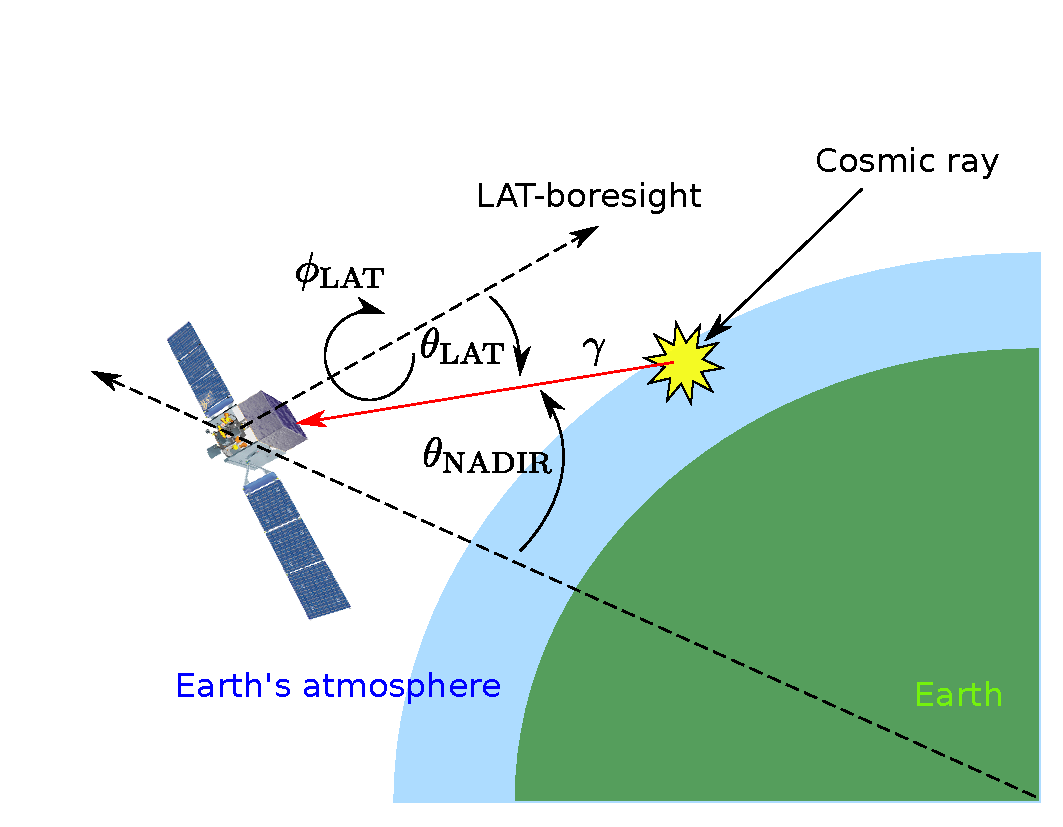
\includegraphics[width=0.7\textwidth]{content/methodology/figures/gamma_production_schematic}
    \caption{
        Schematics of the Earth's $\gamma$-ray production
        from CR interaction with the upper atmosphere.
    }
    \label{fig:gamma_emis_sp}
\end{figure}

Figure \ref{fig:gamma_emis_sp} demonstrates the definitions of some important angular
variables describing a photon's direction in this analysis.
The nadir angle ($\theta_{\rm NADIR}$) is the angle between a
photon's and the nadir direction. The incidence angle
($\theta_{\rm LAT}$) is the angle of a photon's direction with
respect to the detector's boresight. The angle $\phi_{\rm LAT}$
specifies the azimuthal angle of a photon in the LAT's
reference frame.
% The required fundamental concept of spacecraft orientation and 
% the observations of Earth's limb $\gamma$ emission is another crucial
% concept. The Figure \ref{fig:gamma_emis_sp} demonstrates the important
% axis which is $\theta_\text{NADIR}$ represent the angle of how further
% from Earth's center in the spacecraft point of view as well as 
% $\theta_\text{LAT}$ to the angle from incident $\gamma$-ray to the 
% detector normal in the domain between 0 to 90\textdegree
% and $\phi_\text{LAT}$ as the clockwise angle from 0 to 2$\pi$.


\section{Data selection}
In this work, 9 years of
LAT's photon and spacecraft data have been used.
We use the latest version of event reconstruction (Pass 8) with the
cleanest photon event class\footnote{\url{https://fermi.gsfc.nasa.gov/ssc/data/analysis/documentation/Cicerone/Cicerone_Data/LAT_DP.html}}
(ULTRACLEANVETO) in this work.
All data sets can be downloaded pubically
from the LAT's database website\footnote{\url{https://fermi.gsfc.nasa.gov/ssc/data/access/lat}}.

% LAT's flight data has been used
% to analyze reconstructed photon and their metadata of spacecraft
% log recorded in a similar format periodically every half minutes.
% The reconstructed algorithm version is the latest version which is
% Pass 8 with the cleanest photon events that exist from \textit{Fermi}-LAT
% data catalogs called ULTRACLEANVETO. To be more precise, the photon 
% data is collected from publically available raw FITs file from the 

To select the Earth's limb photon produced in the thin-target regime
where the absorption effect could be neglected, we follow the same
criteria ($68.4^\circ < \theta_\text{NADIR} < 70.0^\circ$)
used in the previous LAT analysis by \cite{FermiEarth14}.
We select photons between 10 GeV and 1 TeV which would be
correspond to the CR proton rigidity range of roughly 60 GV
to 2 TV \citep{FermiEarth14}. We also cut photons with
$\theta_{\rm LAT}>70^\circ$ to avoid mis-reconstructions of
large off-axis photons.
% Only high energy limb photon will be selected from 10 GeV up to 1 TeV.
% It makes the traceback analysis for gaining the information of
% CR proton spectrum in rigidity between 60 GV to 2 TV. The definition 
% of $\gamma$-ray's limb region is obtained from \cite{FermiEarth09} in 
% a given nadir angle from 68.4\textdegree to 70.0\textdegree. 
% The maximum of incident angle ($\theta_\text{LAT}$) that was
% measured from the z-axis of the LAT's foresight is 70\textdegree.


\section{Flux extraction}

% There are multiple steps from trivial to the complex calculation to 
% obtain the differential flux. The definition when saying flux 
% is a differential flux that is calculated one
% chunk of energy range at a time as Equation \ref{eq:def_flux}.
The definition of the Earth's limb flux in the energy bin $i$ is given by

\begin{equation}
    \textbf{Flux}(E_i) =  \frac{dN}{dE}(E_i) = \left(\int \frac{\text{Cnt}_i}{\text{Exp}_i}\right) \frac{1}{d(\Omega)dE_i}
    \label{eq:def_flux}
\end{equation}
% \textbf{Flux} \equiv \frac{dN_\gamma}{dE} = \frac{\int_\text{Limb region}(\text{Count map}/\text{Exposure map})}{\Delta\Omega\Delta E}.

where $\text{Cnt}_i$ is the photon count,
$\text{Exp}_i$ is the exposure, $d(\Omega)$
is the solid angle size of the limb region, and $dE_i$ is the energy
bin width. The quantity $\text{Cnt}_i$ and $\text{Exp}_i$ 
are from count and exposure
maps which are discussed in the next subsection.
Since the CR spectrum follows a power law in the energy range
of this analysis, we expect a power law in the Earth's
$\gamma$-ray emission spectrum. Therefore, to calculate the
Earth's $\gamma$-ray spectrum, we divide the energy into 50 bins
eqaully spaced in log scale from 10 GeV to 1.0 TeV.
% Since the CR spectrum follows a power law as the exponential form 
%  $dN/dR \propto R^\gamma$ as mentioned in the background section.
% Then the log-log relation of the flux versus rigidity would behave 
% like a trivial linear trend in the plot. Not only the rigidity but 
% in the high energy CR like 10 GeV also makes the energy of the particle
% almost the same as the rigidity does. Consequently, the $\gamma$-ray
% spectrum is equally divided in the energy space in the log scale for 
% 50 bins.

% To get the spectrum, it is obvious to construct the histogram 
% with 50 bins in a given energy scale as explained in the previous paragraph.
% The flux of each bin could be computed separately by initializing 
% the empty count map and the exposure map where it represents the
% exposure time and the effectiveness of the spacecraft when looking 
% at each angle in the sky. Let regards the following example for 
% a deeper understanding. The ideal scenario is when incident $\gamma$-ray
% walk pass through the LAT in a normal line of the detector. 
% The performance would be the highest it could do.
% On the other hand, if the incident $\gamma$-ray arrives with high 
% tile angle from the LAT's plane (High $\theta_\text{LAT}$).
% An angle resolution is selected to be 2\textdegree in $\phi_\text{NADIR}$
% and 0.1\textdegree in $\theta_\text{NADIR}$. The reason behind these 
% number is simply from the toy experiment of plotting the result 
% in the 2D histogram and it is selected to be the one as the bin value 
% is not too noisy. In another word, it should not be too small so that 
% the result is not too noisy and it is should not so big due to the 
% limb region could not be seen clearly which leads to the matched photon 
% mixed up with the Earth's $\gamma$-rays and collecting too many primaries 
% CR photon.


The flux calculation procedure can be summarized in these following steps.
\begin{enumerate}
    \item Make 2D histograms for which the x-axis is $\phi_{\rm NADIR}$
    and the y-axis is $\theta_{\rm NADIR}$, with 25 bins per
    decade of energy
    \item Select photon data and fill in the 2D histograms
    \item Calculate similar 2D histograms for exposure maps
    which include the effective area
    and livetime of the LAT as it observed the Earth
    \item Compute the flux for each energy bin by
    applying Equation \ref{eq:def_flux}
    % \item Compute the flux by applying Equation \ref{eq:def_flux} in for bin 
    \item Perform background subtraction from an average
    background distribution (Define background in range
    $72.0^\circ < \theta_{\rm NADIR} < 80.0^\circ$)
\end{enumerate}


\subsection{Exposure map calculation}

The exposure map calculation is the most complicated step in
this work because we have to perform coordinate transformation.
In the standard spacecraft data files, the LAT positions and
orientations are recorded in equatorial coordinates.
We have to make a coordinate transformation to obtain the
position of any given pixel in an exposure map in the
spacecraft's reference frame in order to derive the
corresponding effective area for that pixel.
% In fact, step 3 is the most complicated stage in this work.
% Practically, $Fermi$-LAT was designed for observing the space which
% makes the spacecraft logging in equatorial coordinates, not for the 
% Earth's polar coordinates. The LAT position is recorded in equatorial coordinates as well as the LAT's boresight of the detector
% plane to log their orientation during the orbit. At the end of the day,
% the coordinates transformation would be performed from multiple frame 
% of reference to LAT boresight for acquiring the exposure of LAT's FoV
% and reference the effectiveness from LAT's boresight angle dependency.
% The following content is the full detail of how things going on 
% under the hood.

\subsubsection{Coordinate Transformations}

Spacecraft's position and orientation (direction of the
LAT's boresight and solar panel) are recorded in the equatorial
coordinates for which we denote with a symbol ``eq''. We can define
the Cartesian axes for the equatorial coordinate by letting the
x-axis ($\hat{x}_\text{eq}$) point to the vernal equinox for which the right
ascension (RA) is 0$^\circ$ and letting the z-axis point to the
pole for which the declination (DEC) is 90$^\circ$.

We analyze the Earth's $\gamma$-ray emission in the local-zenith
coordinate system denoted by the symbol ``zn,'' as viewed locally
by the LAT.  Here we define that $\hat{x}_\text{zn}$
points along the local
zenith direction of the LAT, and that $\hat{z}_\text{zn}$
points perpendicular
to $\hat{x}_\text{zn}$ in the $\hat{x}_\text{zn}$-$\hat{z}_\text{eq}$
plane. The ``eq'' and ``zn''
coordinate systems are illustrated in Figure \ref{fig:coord_eq_sp}.
Here we assume that $\hat{x}_\text{zn}$ makes an angle 
$\delta_{zn}$ with
the $\hat{x}_\text{eq}$ and $\hat{y}_\text{eq}$ plane,
and $\alpha_\text{zn}$ is the azimuthal
angle of $\hat{x}_\text{zn}$ projection onto
the $\hat{x}_\text{eq}$ and $\hat{y}_\text{eq}$ plane.
% Firstly, the spacecraft orbit is recorded in the equatorial coordinate
% which in a spherical point of view. Defining the cartesian coordinate
% that share the origin between the celestial point of view and the spacecraft 
% by letting one axis point to the spacecraft could assist the calculation
% more conveniently as the Figure \ref{fig:coord_eq_sp}. Please note that 
% the x-axis in the equatorial coordinate is called ``Equinox''.

\begin{figure}[h!]
    \centering
    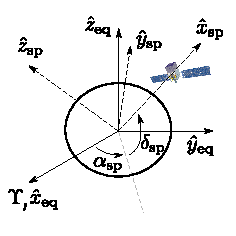
\includegraphics[width=0.5\textwidth]{content/methodology/figures/coord_eq_sp.pdf}
    \caption{
        Illustration of the relationship between the equatorial (eq)
        and local-zenith (zn) coordinate systems for the LAT.
    % Coordinate transform between celestial and spacecraft
    }
    \label{fig:coord_eq_sp}
\end{figure}


% However, mapping into the cartesian 
% coordinate by adopting a unit vector in 3 dimensions has been written
% as Equation \ref{eq:tf_eq_sp} and the synbolic transformation is 
% represented in Equation \ref{eq:rep_tf_eq_sp}.
We can write the components of the zn system in terms of the eq system as

\begin{equation}
    \begin{split}
    \hat{x}_\text{zn} &= \cos\delta_\text{zn}\cos\alpha_\text{zn}\hat{x}_\text{eq} + \cos\delta_\text{zn}\sin\alpha_\text{zn}\hat{y}_\text{eq} + \sin\delta_\text{zn}\hat{z}_\text{eq}\\
    \hat{z}_\text{zn} &= - \sin\delta_\text{zn}\cos\alpha_\text{zn}\hat{x}_\text{eq} + \sin\delta_\text{zn}\sin\alpha_\text{zn}\hat{y}_\text{eq} + \cos\delta_\text{zn}\hat{z}_\text{eq} \\
    \hat{y}_\text{zn} &= \hat{z}_\text{zn} \times \hat{x}_\text{zn}.
    \end{split}
    \label{eq:tf_eq_sp}
\end{equation}

Equation \ref{eq:tf_eq_sp} can be written more
compactly in a matrix form with

\begin{equation}
    \hat{r}_\text{zn} \equiv T_{\text{eq}\rightarrow\text{zn}} (\delta_\text{zn}, \alpha_\text{zn}) \hat{r}_\text{eq},
    \label{eq:rep_tf_eq_sp}
\end{equation}

where $T_{\text{eq}\rightarrow\text{zn}}$ is the transformation matrix which depends on the
values of $\delta_\text{zn}$ and $\alpha_\text{zn}$.
% The transformation matrix $T_{\text{eq}\rightarrow\text{zn}}$ has been implemented as a matrix in practical
% analysis due to the convenience for calculation and the compaction 
% in the programming point of view.


% Unquestionably, it has to be converted into a cartesian point of view to do a mathematical operation for simplicity.
Two variables for determining the LAT boresight
orientation are described 
in equatorial coordinates as declination angle ($\delta_\text{p}$)
and the right ascension angle ($\alpha\text{p}$).
A full representation of the zn and sp coordinates could
be written as Equation \ref{eq:tf_eq_p}.
The compact form is in the Equation \ref{eq:rep_tf_eq_p}.

\begin{equation}
    \begin{split}
    \hat{x}_\text{p} &= \cos\delta^\text{x}_\text{p}\cos\alpha^\text{x}_\text{p}\hat{x}_\text{eq} + \cos\delta^\text{x}_\text{p}\sin\alpha^\text{x}_\text{p}\hat{y}_\text{eq} + \sin\delta^\text{x}_\text{zn}\hat{z}_\text{eq}\\
    \hat{z}_\text{p} &= \cos\delta^\text{z}_\text{p}\cos\alpha^\text{z}_\text{p}\hat{x}_\text{eq} + \cos\delta^\text{z}_\text{p}\sin\alpha^\text{z}_\text{p}\hat{y}_\text{eq} + \sin\delta^\text{z}_\text{zn}\hat{z}_\text{eq}\\
    \hat{y}_\text{p} &= \hat{z}_\text{p} \times \hat{x}_\text{p}
    \end{split}
    \label{eq:tf_eq_p}
\end{equation}

\begin{equation}
    \hat{r}_\text{p} \equiv T_{\text{eq}\rightarrow\text{p}} (\delta^\text{x}_\text{p}, \alpha^\text{x}_\text{p}, \delta^\text{z}_\text{p}, \alpha^\text{z}_\text{p}) \hat{r}_\text{eq}
    \label{eq:rep_tf_eq_p}
\end{equation}

Similarly, $T_{\text{eq}\rightarrow\text{p}}$ is also considered as 
a transformation matrix.
% in the computation for monotizing the source 
% code as well as keeping consistency in the logic.



The LAT coordinate system is defined such that $\hat{z}_\text{sp}$
points along the boresight and $\hat{x}_\text{sp}$ points
along one of its solar panel.
The directions of $\hat{x}_\text{sp}$ and $\hat{z}_\text{sp}$
are also recorded in the
equatorial system. Figure \ref{fig:coord_eq_p} shows the
relationship between the sp and zn coordinate systems.
% Secondly, LAT's boresight coordinates are also referenced in equatorial coordinates. Figure \ref{fig:coord_eq_p} demonstrates the relation between
% an incident plane of the detector on equatorial coordinate and the 
% nadir angle regarding the exposure from LAT to Earth.

\begin{figure}[h!]
    \centering
    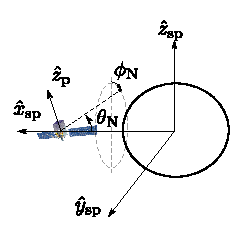
\includegraphics[width=0.5\textwidth]{content/methodology/figures/coord_eq_p.pdf}
    \caption{
        Illustration of the local zenith (zn) and the spacecraft
        (sp) coordinate systems. The nadir ($\theta_{\rm NADIR}$)
        and azimuthal ($\phi_{\rm NADIR}$) angles of a pixel of
        interest is also shown.
    % Coordinate transform between spacecraft and nadir angle
    }
    \label{fig:coord_eq_p}
\end{figure}


With the two transformation matrices,
$T_{\text{eq}\rightarrow\text{zn}}$
and $T_{\text{zn}\rightarrow\text{sp}}$,
we can transform the position of a pixel in a local zenith
coordinate map into the LAT coordinate system to obtain
the effective area for that pixel. The exposure for that
pixel is the sum of effective are $\times$ livetime.
% Again, all those representations just for mapping the LAT's boresight
% coordinate to link with the nadir coordinate to accumulate the 
% exposure from the spacecraft's FoV.
The spacecraft coordinate can be 
written as a dependency of Earth's polar coordinate as Equation \ref{eq:def_r0}
in the cartesian system.

\begin{equation}
    \hat{r}_\text{zn} (\theta_\text{N}, \phi_\text{N}) \equiv -\cos\theta_\text{N}\hat{x}_\text{zn} + \sin\theta_\text{N}\cos\phi_\text{N}\hat{z}_\text{zn} + \sin\theta_\text{N}\sin\phi_\text{N}\hat{y}_\text{zn}
    \label{eq:def_r0}
\end{equation}

Extracting the relations to simplify the 
LAT's boresight coordinate could be contained by one inversion of 
transformation matrix from equatorial to spacecraft and transform it 
to plane of the detector as written in the compact form in the Equation 
\ref{eq:def_r0_to_rp}.

\begin{equation}
    \hat{r}_\text{p} (\theta_\text{N}, \phi_\text{N}) = T_{\text{eq}\rightarrow\text{p}} (\delta^\text{x}_\text{p}, \alpha^\text{x}_\text{p}, \delta^\text{z}_\text{p}, \alpha^\text{z}_\text{p}) \left[T_{\text{eq}\rightarrow\text{zn}} (\delta_\text{zn}, \alpha_\text{zn})\right]^{-1} \hat{r}_\text{zn} (\theta_\text{N}, \phi_\text{N})
    \label{eq:def_r0_to_rp}
\end{equation}

\begin{figure}[h!]
    \centering
    
\includegraphics[width=0.5\textwidth]{content/methodology/figures/coord_plane}
    \caption{
        A vector pointing to a pixel of interest (grey arrow)
        in the plane of detector (p) coordinates.
        The $\hat{z}_\text{p}$ axis
        points along the LAT's boresight
        and the $\hat{x}_\text{p}$ axis
        points along one of its solar panel.
        % Detector's boresight in cartesian and polar coordinate
    }
    \label{fig:tf_lat_pol_car}
\end{figure}

Geometrically, an angular coordinate of the LAT plane could be obtained from
a normalized component of the cartesian unit vector as in Figure
\ref{fig:tf_lat_pol_car}. The exposure accumulation has been
calculated in every single grid from the previous relation.

\subsubsection{Parallel Computations}

The complexity of 
the code becomes large due to the transformation operation.
For example, a plain matrix inversion cost $\mathcal{O}(n^3)$ where 
n is 3 because it is a 3 by 3 matrix in this case.
% Not only the inversion, but
The matrix multiplication also costs the same amount of
complexity
, rendering exposure map calculation a
very computational intensive task.
% which causes a long run in the execution time because 
% the original program has been designed in sequential execution.

The spacecraft files, which contain the information of the LAT
position, orientation, and status in rows of 30-second time step,
are called the FT2 files. We use 25 energy bins per decade,
so the bin width is small enough to use the geometric mean
to represent the mean energy for each bin. 
Moreover, the exposure maps can be calculated separately
for a given time period. We can therefore split the
9-year analysis time into many small time periods,
calculate the exposure maps for each time period
in parallel, and sum all periods to obtain
the total exposure maps.
% Nevertheless, the spacecraft log file namely ``FT2'' has been recorded
% row by row which equivalently to a CSV format as a plain table with 
% the specific columns. Since the objectives are to determine the exposure map
% by counting the exposure time as well as the effectiveness of the spacecraft 
% from each angle for a given small range of energy which means that 
% the energy could be approximate as one energy for getting the effective 
% area in each angle of the LAT during calculation. Moreover, the exposure 
% could be calculated parallelly for each step or in each row of the FT2 due to 
% the property of the exposure map. Consequently, splitting the exposure map 
% and calculate parallelly is possible to get rid of the performance issue.

The code is implemented
in Message Passing Interface (MPI). The framework provides 
a simple protocol for communicate between each process
with a customizable message schema.
It assists the user to 
freely control multiple processes with full control of 
each process. According to Flynn's taxonomy of computation,
this work exploits the Multiple Instruction Multiple Data (MIMD)
architecture to utilize the resources in a distributed system.

\begin{figure}[h!]
    \centering
    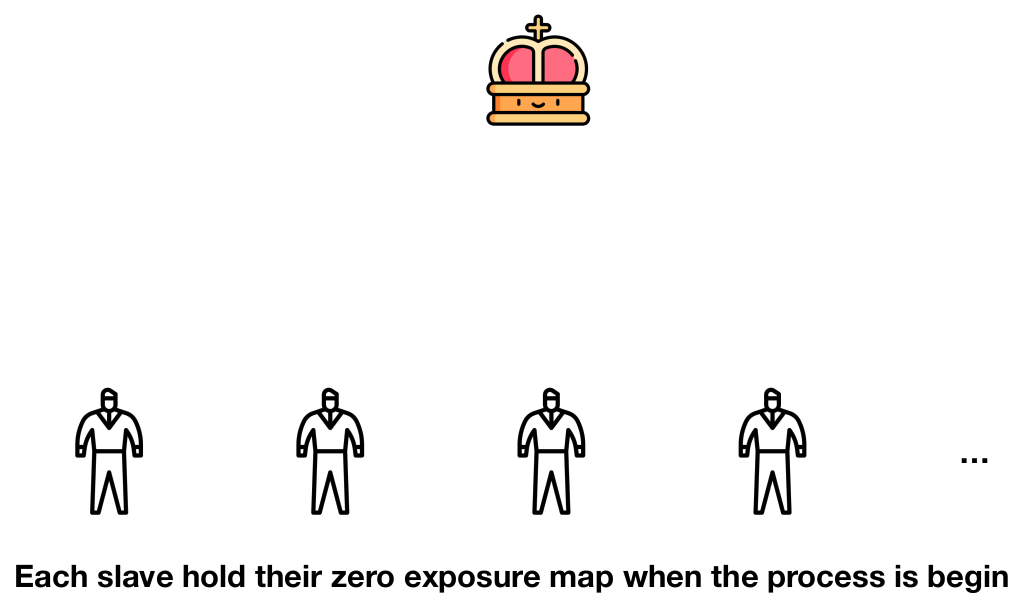
\includegraphics[width=0.7\textwidth]{content/methodology/figures/ms1_v2}
    \caption{Spawning the king and slave processes}
    \label{fig:ms1}
\end{figure}

In the normal parallel computing setup, sending equal
amount of task to each node is not optimized since
there would be fast and slow nodes with different performances. 
Some trivial tasks can lock resources in a
computing cluster and blocks the resource
allocation for other tasks. 
% To begin with, the calculation, initializing the exposure map with a 
% separate workers and send multiple rows to the workers in the same amount
% is trivial and waste a lot of resources since there will be a fast worker 
% who do a calculation fast and the slow worker due to the cluster 
% is composed of non-monolithic nodes with different performances.
% The trivial calculation will lock the resource in the cluster and blocks 
% the other researcher who wants to run because of the resource allocation issue.
To maximize the usage of the CPU-based cluster computing, there is a 
mechanism called the ``Master-Slave technique''. The algorithm has been designed for utilizing the resource by spawning a king as the process manager 
and multiple slaves to be process workers. The starting process could 
be demonstrated in Figure \ref{fig:ms1}. 


\begin{figure}[h!]
    \centering
    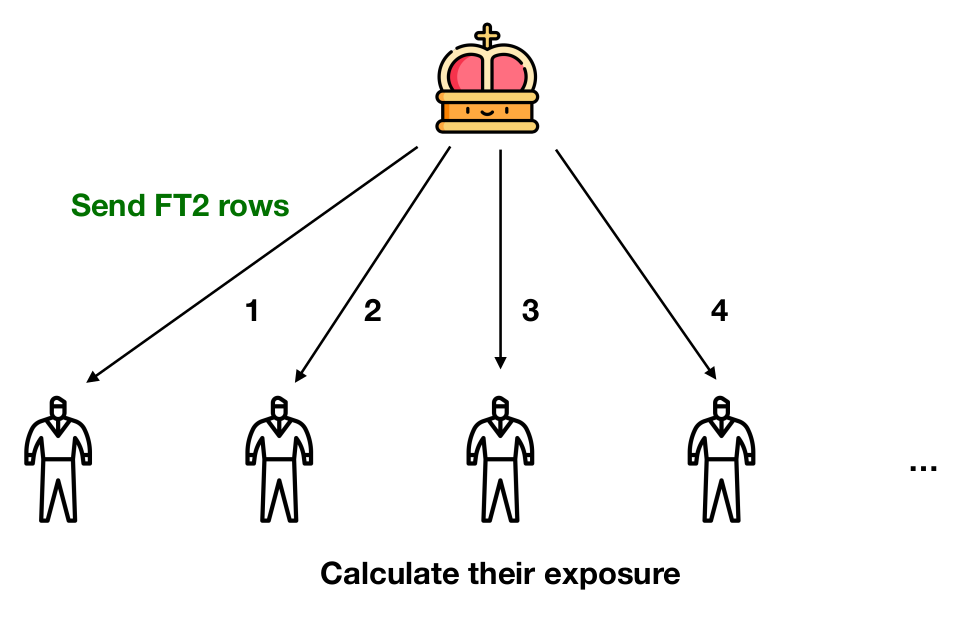
\includegraphics[width=0.7\textwidth]{content/methodology/figures/ms2}
    \caption{Master process sends a small task to slaves.}
    \label{fig:ms2}
\end{figure}


\begin{figure}[h!]
    \centering
    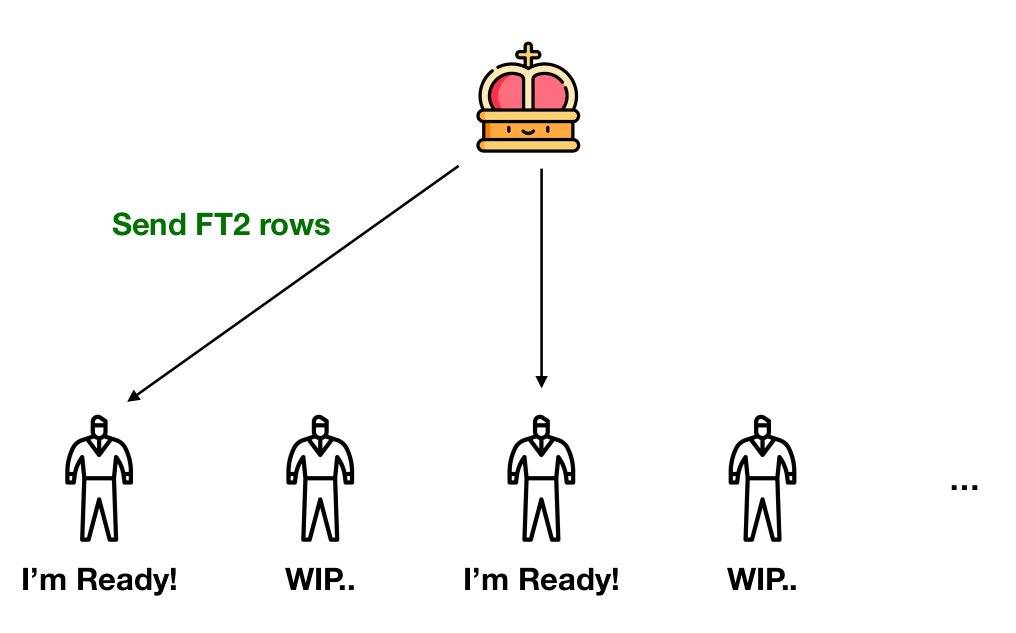
\includegraphics[width=0.7\textwidth]{content/methodology/figures/ms3}
    \caption{Asynchronous assignment of tasks to available slaves.}
    \label{fig:ms3}
\end{figure}

A certain amount of spacecraft information (FT2 rows)
would be sent as an input to slaves sequentially
until all slaves are assigned with a small task
and start the calculation.
% After that, the FT2 rows will be sent to slaves sequentially until
% all workers hold a small chunk of data and do their jobs.
There are metadata attached
% In practice, there is metadata attach
to the message. 
One of the options is the status tag
which let the slaves declare the status of a process
% The status tag sends to the worker to declare the state of the process
whether it is still in process or has finished.
Figure \ref{fig:ms3} illustrates 
the non-sequential assignment of the workload.
Small tasks are sent to available slaves and skip busy slaves.
% The idea is simply sending a small task to an available worker and skip a busy worker
% without disturbing them.
This mechanism allows the execution to utilize 
the resource in the cluster without wasting
free slaves. After all tasks are assigned,
the master process will send a status tag announcing
that the overall calculation has finished.
Then, the exposure maps from all slaves would be added
to obtain the final total exposure maps.
Examples of master-slave calculation are shown in Appendix \ref{appendix:exposure}.
% in the free worker.


% By the end of the day, if the task is completely sent.
% The master process will send the status tag as done to be an 
% announcement of the finishing period. Then the exposure map of 
% each worker will be gathered in the master process for superposition
% and dump it to unify an exposure map. In addition, the calculation 
% in an early period of testing is reported in Appendix \ref{appendix:exposure}.


\section{Hadronic Collision Model}
CR spectrum is well described in power in ridigity where 
the ridigity is a momentum per charge of the particle.
The explicit formula for proton power-law spectrum in rigidity
in Equation \ref{eq:spl} as a single power law (SPL)
where $\Gamma$ represents the spectral index of the model. 
% In fact, the spectrum has been observed as the differential flux 
% in energy.
Converting between the ridigity ($R$) and the 
energy spectrum is derived in Appendix \ref{appendix:pw_energy}.


\textbf{Single power law (SPL)}
\begin{equation}
    \frac{dN}{dR} = R_0R^{-\Gamma}
    \label{eq:spl}
\end{equation}

where $R_0$ is the coeffient of the powerlaw.
The most crucial part of this work is to determine if there is any 
breaking in the spectral index of the power law. To represent 
a single breaking energy, the broken power law (BPL) could be modeled 
by Equation \ref{eq:bpl}. 


\textbf{Broken power law (BPL)}
\begin{equation}
\frac{dN}{dR}=
  \begin{cases}
    R_0R^{-\Gamma_1}\ :\ E < E_{\text{Break}}\\
    R_0[R(E_{\text{Break}})]^{\Gamma_2-\Gamma_1}R^{-\Gamma_2}\ :\ E \ge E_{\text{Break}}
  \end{cases}
  \label{eq:bpl}
\end{equation}

% The scattering process of the hadronic collision from proton hitting 
% the atmospheric molecules.
The collision from incoming protons with kinetic 
energy above 10 GeV striking the Earth's atmosphere
be modeled by proton-proton collision with 
with the scaling of normalization depending
on the chemical composition of the air.
% an approximation that depends on the majority of the air components.
The proton-proton collision yielding $\gamma$ rays
as secondary products for a broad and smooth spectrum
of proton can be modeled by Equation \ref{eq:KO_model}
taken from \cite{K&Omodel} as 
% Model for the collision of proton-proton which yields $\gamma$-ray 
% as a secondary product as a distribution in the spectrum has been 
% derived in
% Equation  from \cite{K&Omodel} work.

\begin{equation}
    \frac{dN_\gamma}{dE_\gamma} \propto \int^{E_{\text{max}}}_{E_\gamma} dE'\frac{dN_p}{dE'} \frac{d\sigma^{pp\rightarrow\gamma}(E',E_\gamma)}{dE_\gamma},
    \label{eq:KO_model}
\end{equation}

where $d\sigma^{pp\rightarrow\gamma}(E',E_\gamma)/dE_\gamma$ contains 
the scattering amplitude
for the kinetic energy of proton $E'$ and the
energy of $\gamma$ ray $E_\gamma$.
% of a given kinetic energy proton and the spectrum of the $\gamma$-ray.
Atmospheric components mostly consists 
of nitrogen as the majority and the oxygon \citep{atmosCompos}. The cross-section from 
proton-proton collision and proton-nitrogen collision is roughly 
approximate as the multiplicative relation since there is plateau 
curve in the energy range in this analysis. The relation of the proton-proton 
scattering amplitude and the proton-nitrogen is obtained from \cite{WAtwater}
where it highly depends on the atomic numbers of the air molecules. 

However, the second highest fraction of the arrival CR particles on 
Earth is an alpha ($\alpha$) particle. The helium nuclei can interact with the nitrogen and produce high energy $\gamma$-rays depends on
how much kinetic energy $\alpha$-particles is holding. Another 
estimation has been exploited by applying $\sigma_{\alpha N}/\sigma_{pN}$
to be a constant around 1.6 at the energy range in GeV from 
the same relationship of the proton-air collision model. Hence, derived
equation of the scattering process from incoming 
proton and $\alpha$-particle with air molecules to produce $\gamma$-ray
spectrum could be shown as Equation \ref{eq:derived_model}

\begin{equation}
    \frac{dN_{\gamma}}{dE_\gamma}(E_\gamma) \propto
    \sum_{E'_i}\left[\frac{E'_i}{E_{\gamma}}\Delta(\ln E'_i) \right]
    \left[ 
        f_{pp}\frac{dN_p}{dE'_i}
        \left\{
            1+\frac{\sigma_{\text{HeN}}}{\sigma{p\rm N}}\left(\frac{dN_p}{dR}\right)^{-1} \frac{dN_{\text{He}}}{dR} \frac{dR_{\text{He}}}{dR_p} 
        \right\}
    \right]
    ,\label{eq:derived_model}
\end{equation}

The CR helium spectrum would not be measured in this work since there will be multiple parameters that leads to an overwhelming 
local optimum. The spectrum of $\alpha$-particles is directly measured 
by \cite{AMS-02Helium} and fix the distribution as one function rather 
modeled spectrum of CR proton spectrum. The full detail of the 
equation derivation will be demonstrated in \ref{appendix:interaction_model}.


% Eventhough converting process requires a derivation, the energy
% and ridigity of the proton particle could be approximate as the 
% same number for the lesser operation. Since the proton mass energy 
% is around 0.938 GeV/c$^2$. 

\section{Optimization}
Determining the best-fit spectral model requires an objectives function
to represent how well the model match with an observed data. A proper 
methodology for fitting or optimization in another word is also 
a crucial part since it is likely that the local optimum exists in the parameters space. A poor optimization could lead the best-fit
stuck in a local minimum and yield a poor result. For better escaping 
local optima, heuristic optimization is employed for finding the 
best-fit of the model in parameter space.


\subsubsection{Poisson likelihood function}
An objective function is defined as Poisson likelihood function 
in the Equation \ref{eq:likelihood}. The reason behind the selection 
of the Poisson function came from the observed model and measurement is 
considered as a number of photons in each bin of the histogram. 
Converting the model spectrum to be a count histogram is simply
multiplied by the integral of the exposure map in the limb region.

\begin{equation}
    \mathcal{L} = \prod_{i=1}^{N} P_{\text{pois}}(n_{\text{i,model}}, n_{\text{i,measurement}})
    \label{eq:likelihood}
\end{equation}

Since the spectrum order is in different order of magnitude, then a
proper way to define an objective function is to redefine a
likelihood as a log-likelihood function for numerically
convenient like Eq \ref{eq:loglikelihood}. 

\begin{equation}
    Sum = \sum_{i=1}^{N} -\log P_{\text{pois}}(n_{\text{i,model}}, n_{\text{i,measurement}})
    \label{eq:loglikelihood}
\end{equation}

To sum up, a given proton spectrum yield a distribution of $\gamma$-ray
spectrum to be converted into a count histogram and comparing with the 
real measurement. Not only for numerical convenient but the negative sign 
also makes an algorithm to minimize the system rather than maximize 
a likelihood.

\subsubsection{Particle Swarm Optimization (PSO)}

In the early phase of the optimization, a plain gradient descent 
optimization has been used for model fitting. The result turns out 
that with different initial parameters, the different best-fit model 
has changed which implies the local minimum in the problem. 
Even there is no method to guarantee the global minimum but the heuristic
optimization could be a better option for handling this type of problem.
One kind of most widely used algorithm is particle swarm
optimization (PSO) and it is invented by \cite{pso_optimize}.

In order to get a best fit spectral indices, employing the Particle Swarm Optimization (PSO)
by randomly initiate many particles in a given range of the parameter space and find the
local and global best fit in each step of the iteration. Then rest of them would slowly move
toward to the local and global position in parameter space with a proper weight. 
The iteration process will stop when the standard deviation of the objective function from 
every particle less than a decimal. The explicit formula for every iteration $k$,
particle $i$ move with velocity $v_k^i$ is

\begin{equation}
    v^i_{k+1} = \omega v^i_k + c^br^b_k[b^i_k-x^i_k] + c^Br^B_k[B^i_k-x^i_k],
    \label{eq:pso}
\end{equation}
and updating the particle $i$ with
\begin{equation}
    x^i_{k+1} = x^i_k + v^i_{k+1}.
    \label{eq:pso_update}
\end{equation}
where
\begin{itemize}
    \item $x^i_k$ represent variable that particle $i$ hold
    \item $b$ and $B$ are best local and global parameter sets along the optimization process
    \item Set $\omega = 0.2$, $c^b = 0.2$ and $c^B = 0.3$
\end{itemize}

\section{Statistical significance}

Certainly, larger model parameters or complexity would yield 
a better performance except it is overfitting the problem.
The critical issue is to answer how much significance the alternative 
model could outperform the trivial model. As the language of statistics 
would consider as two hypotheses. One for null and one for alternative 
approach. 

For this case, BPL has 2 more degrees of freedom (DOF) than SPL.
Unquestionably, if there is a good optimization procedure, 
the objectives function would say BPL is better SPL. As mentioned 
from the previous paragraph, the significance level has to be taken
into account to put the weight on the study. Theoretically, regarding 
the model likelihood with a given set of parameters could be determined 
in the general case as Wilk's theorem define the relation in 
Equation \ref{eq:wilk}.

\begin{equation}
    \mathcal{L} \equiv \prod_{\alpha=1}^n f(x_\alpha, \theta_1, \theta_2, ..., \theta_h)
    \label{eq:wilk}
\end{equation}
where 
\begin{itemize}
    \item $x_\alpha$ is represent a variant from model and data
    \item $\theta_i$ is a degree of freedom (DOF)
\end{itemize}

The practical usage to compare the null hypothesis and the alternative 
hypothesis as similar to one-tail hypothesis testing with a given 
dependency in more DOF has been adopted by \cite{Huelsenbeck}.
This method called ``Likelihood ratio test (LRT)''. The compact formula 
is shown in Equation \ref{eq:lrt}.

\begin{equation}
    \text{LRT} = -2\ln\left(\frac{\mathcal{L}_\text{null}}{\mathcal{L}_\text{alternative}}\right)
    \label{eq:lrt}
\end{equation}


% \section{Error Determination}

% Monte Carlo Simulation







% \lofcont


\chapter{Results and discussion}

The content of this chapter would be reported as the analysis 
procedure from step one to the end. The first part is the data 
correction process, count maps from the raw count as well as 
exposure map from the parallel computation, the spectrum and 
inversive fitting from heuristic optimization.

\section{Limb's angle correction}
Theoretically, the peak profile of the $\theta_\text{NADIR}$ would be
the same when time passes by.
From the observations, the nadir angle change through time 
evolving since the spacecraft altitude is gradually getting lower
in each year which will affect the LAT point of view when it sees 
the Earth.

\begin{figure}[h!]
    \centering
    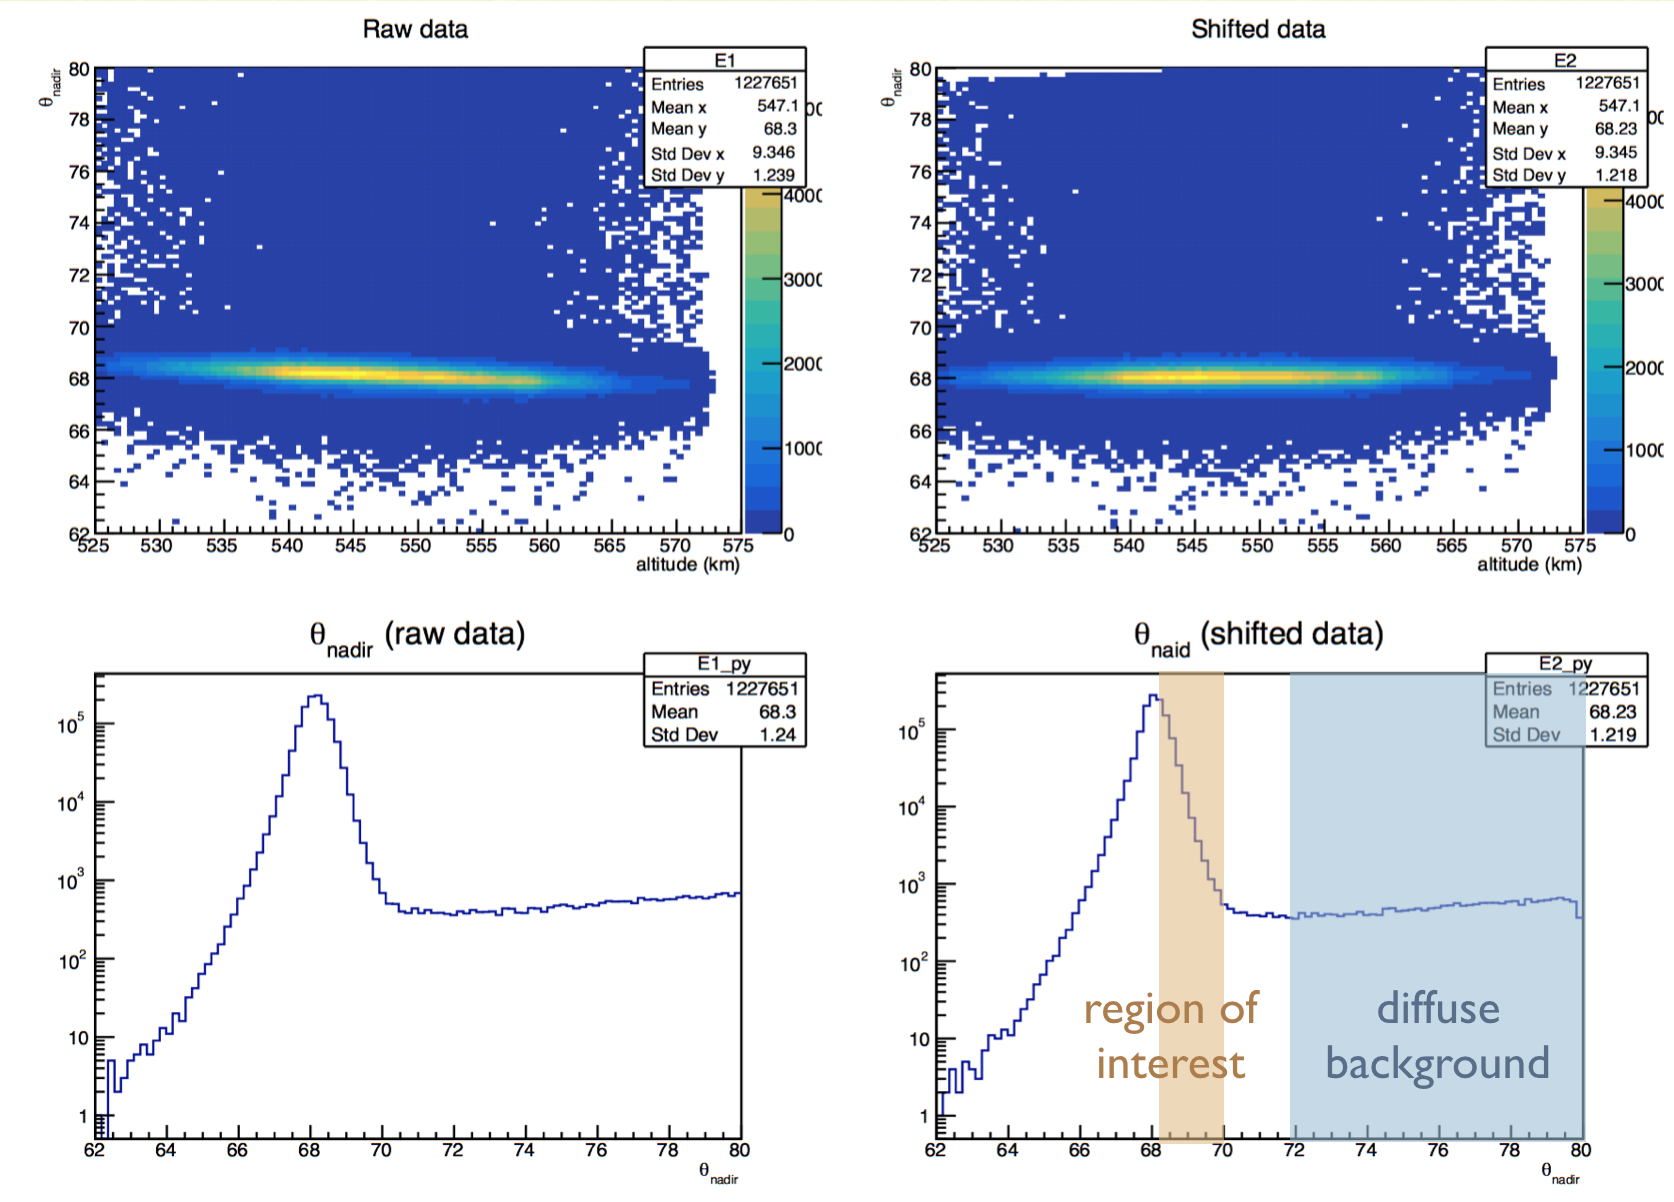
\includegraphics[width=0.8\textwidth]{content/result_and_discussion/figures/LATShifted.png}
    \caption{
        Distribution of nadir angle before and after altitude correction.
        (top) Heatmaps represents the photon density in axis
        of $\theta_\text{NADIR}$ versus altitude in kilometers.
        The left one came from raw data and the right one was
        converted by altitude shifting calculation.
        (bottom) The projected histograms from the above heatmaps
        in the axis of $\theta_\text{NADIR}$ where all photon
        from various altitudes was accumulated into the bin value.
    }
    \label{fig:lat_nadir_shifted}
\end{figure}


The top-left of Figure \ref{fig:lat_nadir_shifted} demonstrates how 
much spacecraft orbiting altitude correlate to the $\theta_\text{NADIR}$
by a 2D heatmap plot of photon intensity. The bottom-left histogram
came from the projection of the previous raw count 2-D histogram which 
has a peak around 68\textdegree. Both bottom and top right histograms
was constructed from the same logic but there is one different 
variable. The shifted nadir angle has been calculated to reduce the 
effect from the spacecraft and the region of interest has been highlighed 
as orange for calculating as the limb spectrum and the blue zone is 
a diffusive background to be used in the background subtraction.

The brightness of Earth's limb is much brighter than the 
diffusive background on the map. The region of interest and 
the background intensity has a huge difference in approximately
an order of magnitude.


\section{$\gamma$-ray spectrum measurement}

According to the definition from Equation \ref{eq:def_flux}, 
the first step is the construction of the count map of the Earth's 
centered coordinates. To illustrate how the outcome looks like,
we selected photon data from a single week due to the raw data
of photon from \textit{Fermi} was published once a week as one file.
A week of the accumulated photons is plotted in
the Figure \ref{fig:sample_photon_dist} to visualize 
the raw count of the sample data on the count map.

\begin{figure}[h!]
    \centering
        \subfloat[
            Heatmap of photon density in nadir angle where the 
            radius direction is the azimutal nadir
            angle ($\theta_\text{NADIR}$).
        ]{
            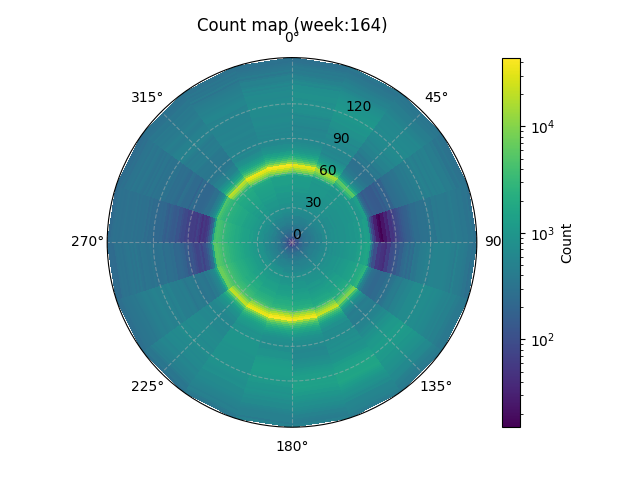
\includegraphics[width=0.47\textwidth]{content/result_and_discussion/figures/cntmap_polar.png}
        }
        \hfill
         \subfloat[
            A projected histogram from the heatmap.
            The x-axis is $\phi_\text{NADIR}$ from 0\textdegree
            to 360\textdegree.
        ]{
            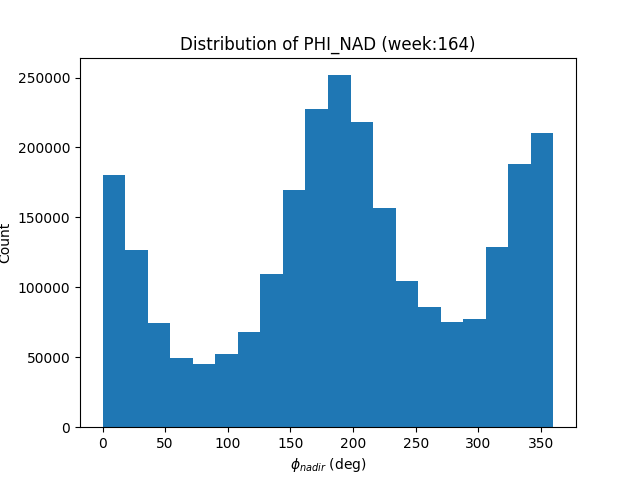
\includegraphics[width=0.47\textwidth]{content/result_and_discussion/figures/phi_nad_dist.png}
        }
        \caption{An example distribution of $\gamma$-ray from a single week.}
       \label{fig:sample_photon_dist}
\end{figure}

The limb's region could be easily observed in the bright ring above 
a dashed line of 60\textdegree $\theta_\text{NADIR}$.
Figure \ref{fig:sample_photon_dist} also shows the brightness of 
the southern and northern hemispheres. Further investigating of the 
East-West effects could be illustrated by projecting the 2-D histogram 
into a 1-D histogram of the nadir angle as in Figure \ref{fig:sample_photon_dist}b.
Nevertheless, the explanation of the East-West is a rough description
and still incomplete because it does not take
the exposure into account yet.

% Applying criteria from the data selection such as event class,
% LAT's incident angle would affect the result from
% the histogram filling.


\begin{figure}[h!]
    \centering
    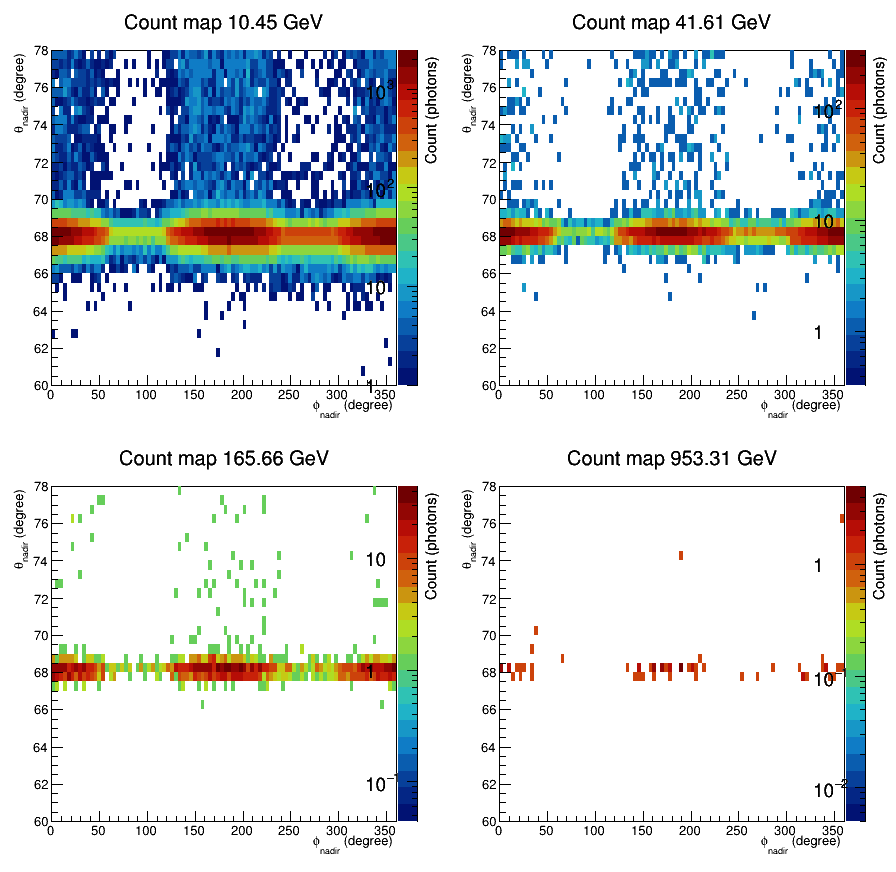
\includegraphics[width=0.8\textwidth]{content/result_and_discussion/figures/cartesian_cntmaps.png}
    \caption{
        Cartesian plot of the $\gamma$-ray count histograms.
        The title is each sub-figure represent
        mean of the energy bins.
    }
    \label{fig:cntmap_cartesian}
\end{figure}

Since the final spectrum will contain 50 energy bins
with their specific energy range and mean energy
for each energy bin.
In practice, each heatmap will be constructed
for their belonging bin of the histogram in the energy domain
as in the Figure \ref{fig:cntmap_cartesian}.


However, inspecting at polar coordinate plotting
from the cartesian point of view might not be the best option for 
illustration since it not looks like the real orientations.
Figure \ref{fig:cntmap_polar} is another
angle of viewing the same data but in more natural orientations.
Both visualizations show that the Earth's limb region in $\gamma$-ray 
is the shinest band for all interesting energy.
It is also obvious to say that the higher energy scale,
the less photon appears after applying criteria.


\begin{figure}[h!]
    \centering
    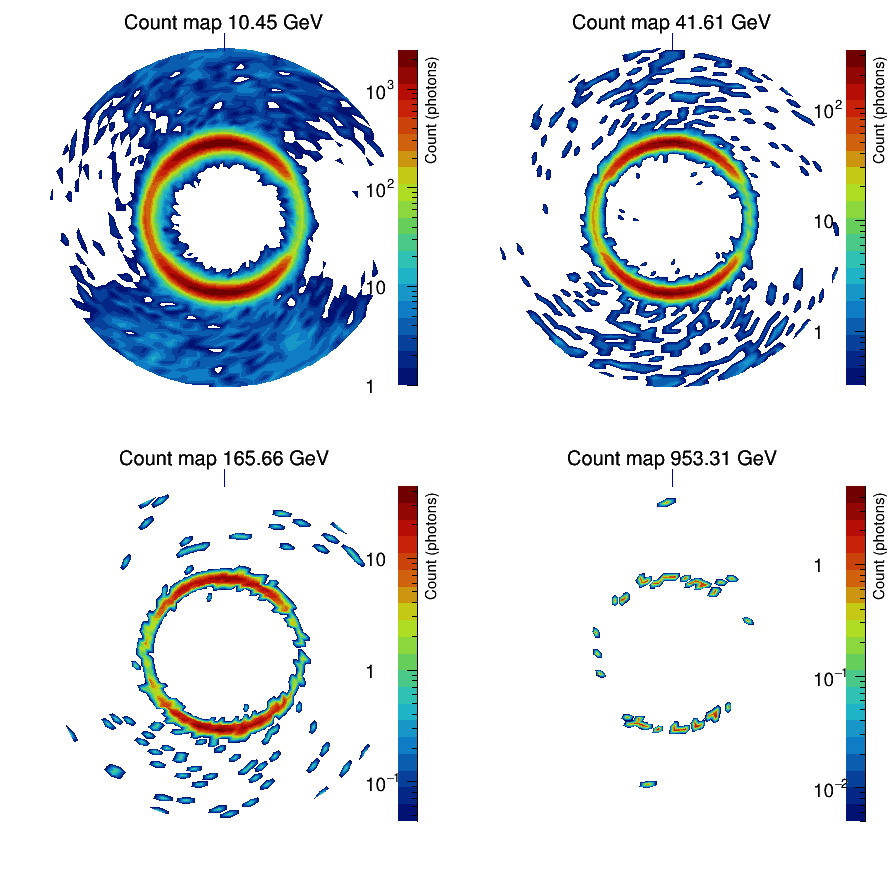
\includegraphics[width=0.8\textwidth]{content/result_and_discussion/figures/polar_cntmaps.png}
    \caption{Polar plot of the $\gamma$-ray count histograms.}
    \label{fig:cntmap_polar}
\end{figure}


The next step is the exposure calculation.
The exposure map is computed 
by accumulating exposure time from the LAT's FoV
in each step time as well as takes the 
effectiveness of the detector due to incident angle
affects the performance of the detector.
A unit from the calculation will be an 
area multiple by the time. Raw cartesian plots are visualized in
Figure \ref{fig:expmap_cartesian} with an attached axis.

\begin{figure}[h!]
    \centering
    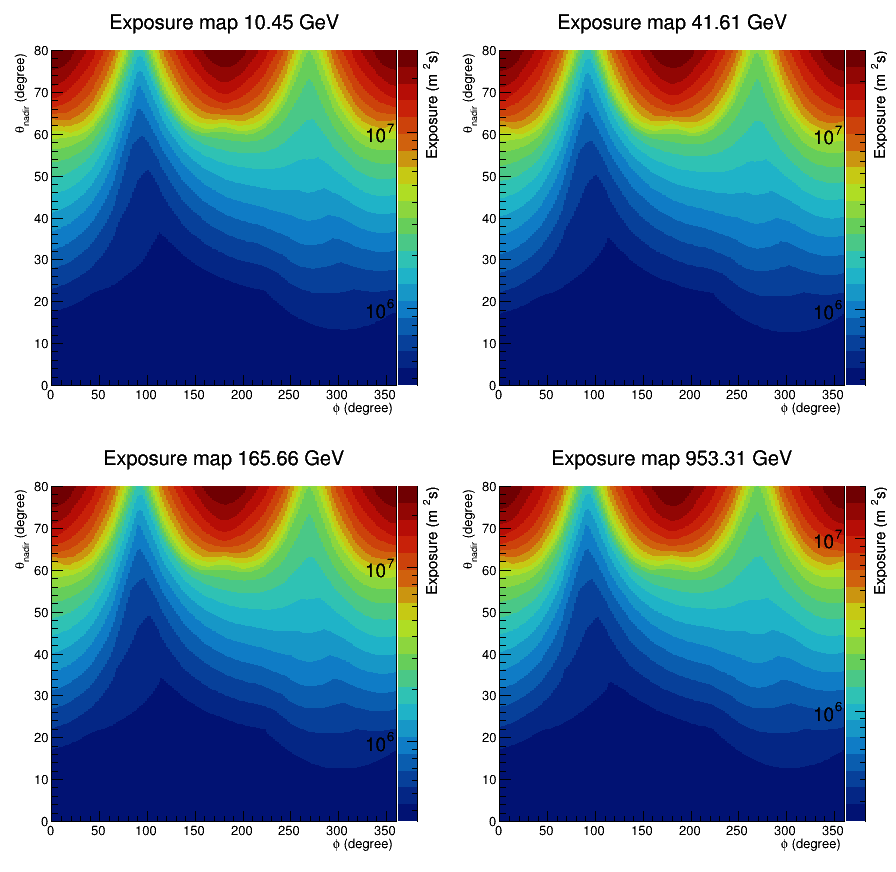
\includegraphics[width=0.8\textwidth]{content/result_and_discussion/figures/cartesian_expmaps.png}
    \caption{Cartesian plot of the exposure histograms.}
    \label{fig:expmap_cartesian}
\end{figure}


The exposure intensity in the sky is much
higher than the Earth in an order of magnitude
because \textit{Fermi} was designed
for seeking flare events in space rather than the Earth.
Regarding a given nadir angle between
60\textdegree to 70 \textdegree,
the spacecraft seems to look at the northern and southern hemisphere 
more than the eastern and the western side. The color of the 
at 270\textdegree (West) is more intense than 90\textdegree (East)
means that the spacecraft tends to peek in the Westside more
than Eastside. The reason might come from the
trajectory of the charged particles was bent
and produce a $\gamma$-ray which potentially could 
convince \textit{Fermi} to look at them rather
than the other side because it 
has a more for triggering the GBM.
The 2-D histograms in polar coordinates have also been
plotted in Figure \ref{fig:expmap_polar}.

\begin{figure}[h!]
    \centering
    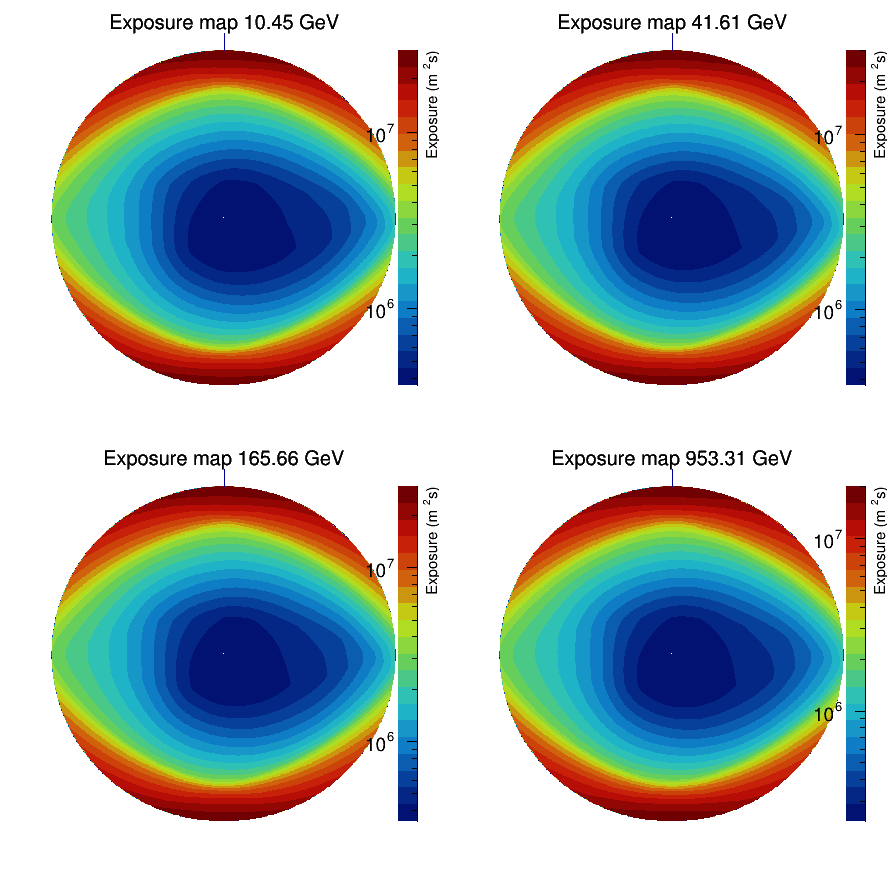
\includegraphics[width=0.8\textwidth]{content/result_and_discussion/figures/polar_expmaps.png}
    \caption{Polar plot of the exposure histograms.}
    \label{fig:expmap_polar}
\end{figure}


The last step starts with initiating the new heatmaps that were 
defined by the element-wise division from the
count maps and the exposure maps.
After that, integrating the limb region in the polar coordinates
to get a single scalar value. The scalar is then divided by the 
gap of the energy bin and the solid angle.
Repeating the above process for 50 energy bins in the $\gamma$-ray 
spectrum and subtracts by the background would yield the final 
photon spectrum as in Figure \ref{fig:flxhist}.

\begin{figure}[h!]
    \centering
    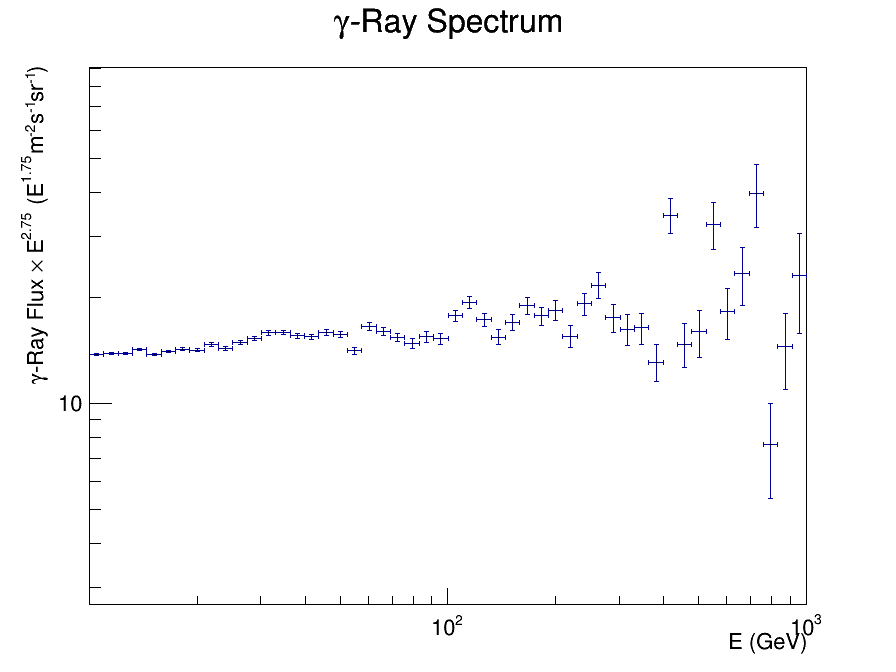
\includegraphics[width=0.7\textwidth]{content/result_and_discussion/figures/flx_hist.png}
    \caption{Measured $\gamma$-ray spectrum.}
    \label{fig:flxhist}
\end{figure}

In addition, exploring the $\gamma$-ray
intensity from the visualization
of the Earth's centered coordinates would be informative aspects
to observe the variation of the photon
intensity along the nadir angle as well as the 
East-West effect. The cartesian plotted is in Figure
\ref{fig:flxmap_cartesian} and the polar form as in the Figure 
\ref{fig:flxmap_polar}. Comparing the intensity along the peak of 
theta nadir in the cartesian plot from the East ($\phi$=90\textdegree)
and West ($\phi$=270\textdegree) would reflect that the band of 
the intensity in the west is slightly
thicker than in the East and the 
color of the peak center is more a little darker than the other 
side. It means that not only the intensity
but also the ring thickness
of the limb region is larger from West to East.


\begin{figure}[h!]
    \centering
    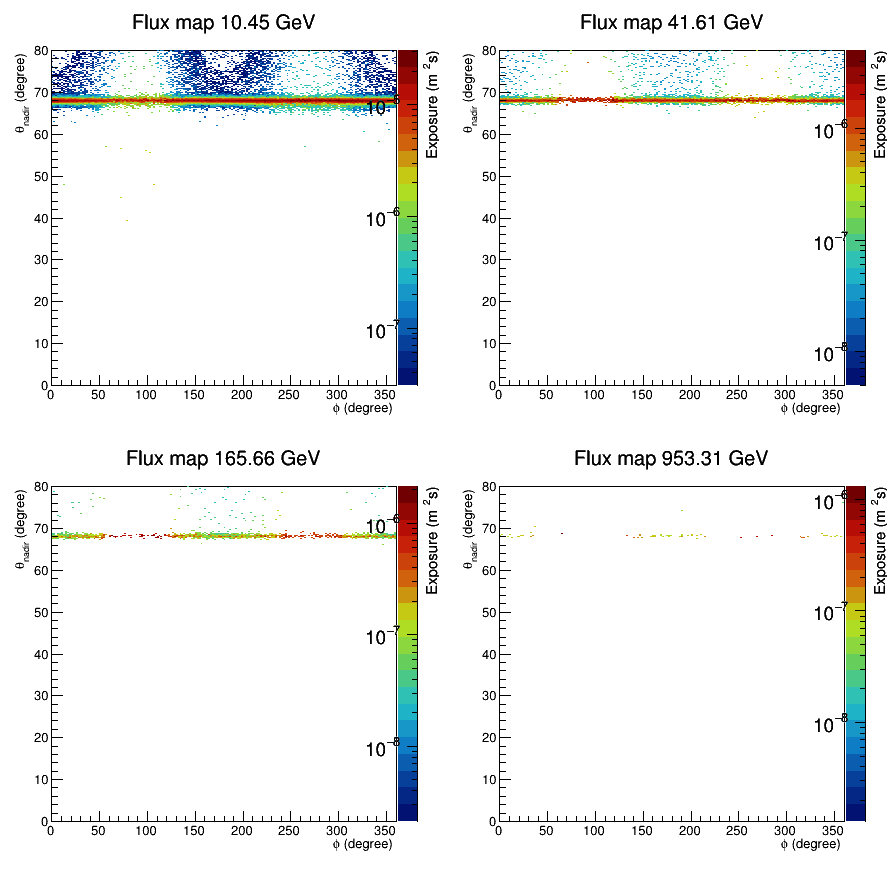
\includegraphics[width=0.8\textwidth]{content/result_and_discussion/figures/cartesian_flxmaps.png}
    \caption{Cartesian plot of the $\gamma$-ray flux histograms.}
    \label{fig:flxmap_cartesian}
\end{figure}


\begin{figure}[h!]
    \centering
    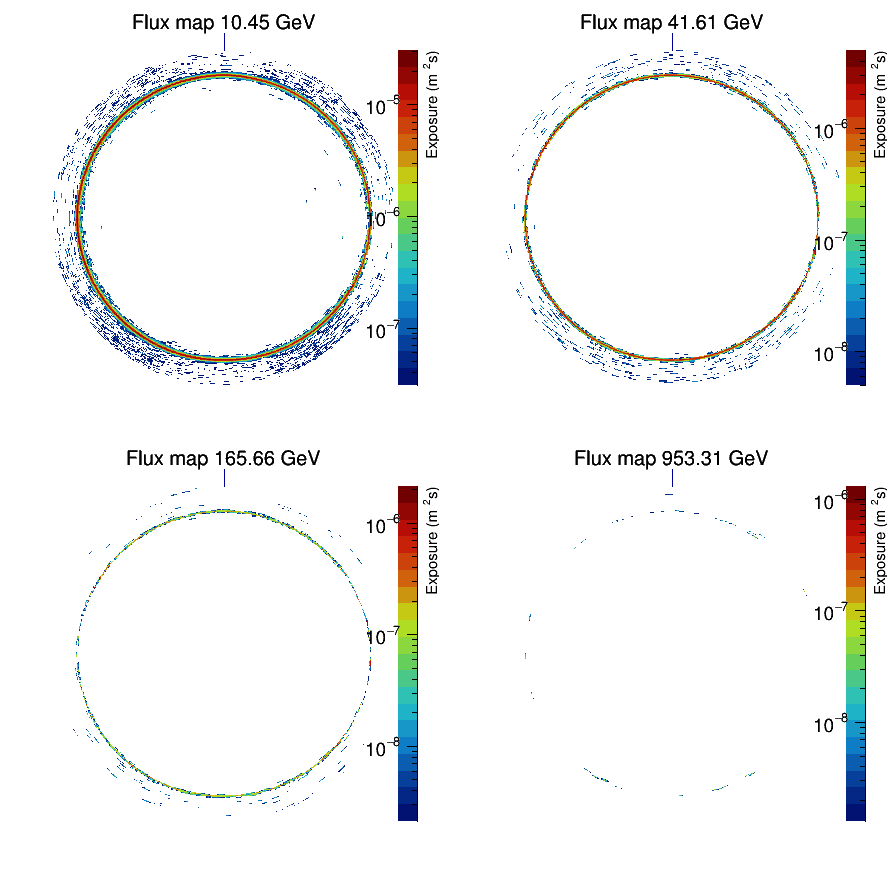
\includegraphics[width=0.8\textwidth]{content/result_and_discussion/figures/polar_flxmaps.png}
    \caption{Polar plot of the $\gamma$-ray flux histograms.}
    \label{fig:flxmap_polar}
\end{figure}

\newpage

\section{Best fit result}

The optimized parameters for SPL and BPL models are summarized in 
Table \ref{tb:bestfit}. Best fit $\gamma$-ray from both models are 
visualized in the Figure \ref{fig:fitted_gamma_specgtrum} along
with spectrum from the measurement. The result shows the consistency
between the direct measurement from AMS-02 and
the previous work. Both studies identify the breaking point 
of the spectral index in proton spectrum at $\sim$ 300 GeV as well 
as the previous work reported $\Gamma_1 \sim 2.81$
and $\Gamma_2 \sim 2.68$ for the BPL model.

\begin{table}[h!]
    \centering
    \begin{tabular}{l | c | c | c}
      Best fits & $\Gamma_1$ & $\Gamma_2$ & $E_{\text{Break}}$ (GeV) \\
      \hline \hline
      SPL & 2.70 & - & -  \\
      BPL & 2.86  & 2.63 & 333
    \end{tabular}
    \caption{Optimization results.}
    \label{tb:bestfit}
\end{table}

The comparative illustration
also be visualized in the Figure \ref{fig:fitted_cr_proton} with a 
scaled spectra from both models to collate two other direct 
observations of the space-based experiments. It is obvious to see 
the consistency of BPL with the direct measurements in the bellowing 
sub-figure is more corresponding than the SPL model in the top sub-figure
because the breaking point of the BPL does looks more likely to be 
a proper model where the x-axis is the same rigidity scale.

However, a more complex model would perform better than the model 
that has less degree of freedom in practice. Determining the 
statistical significance would be the best way to answer whether 
CR spectrum is naturally described as a BPL indeed.
The significant level could be determined by
taking the outcome from the objective function
to Equation \ref{eq:lrt} for testing one-tail hypothesis-like
from the null hypothesis comparing to an alternative
hypothesis which is the model of breaking of spectral indices
, or SPL versus BPL in other words.
The significance is around 1.38$\sigma$ or
at 92\% confidence level.


\begin{figure}[h!]
    \centering
    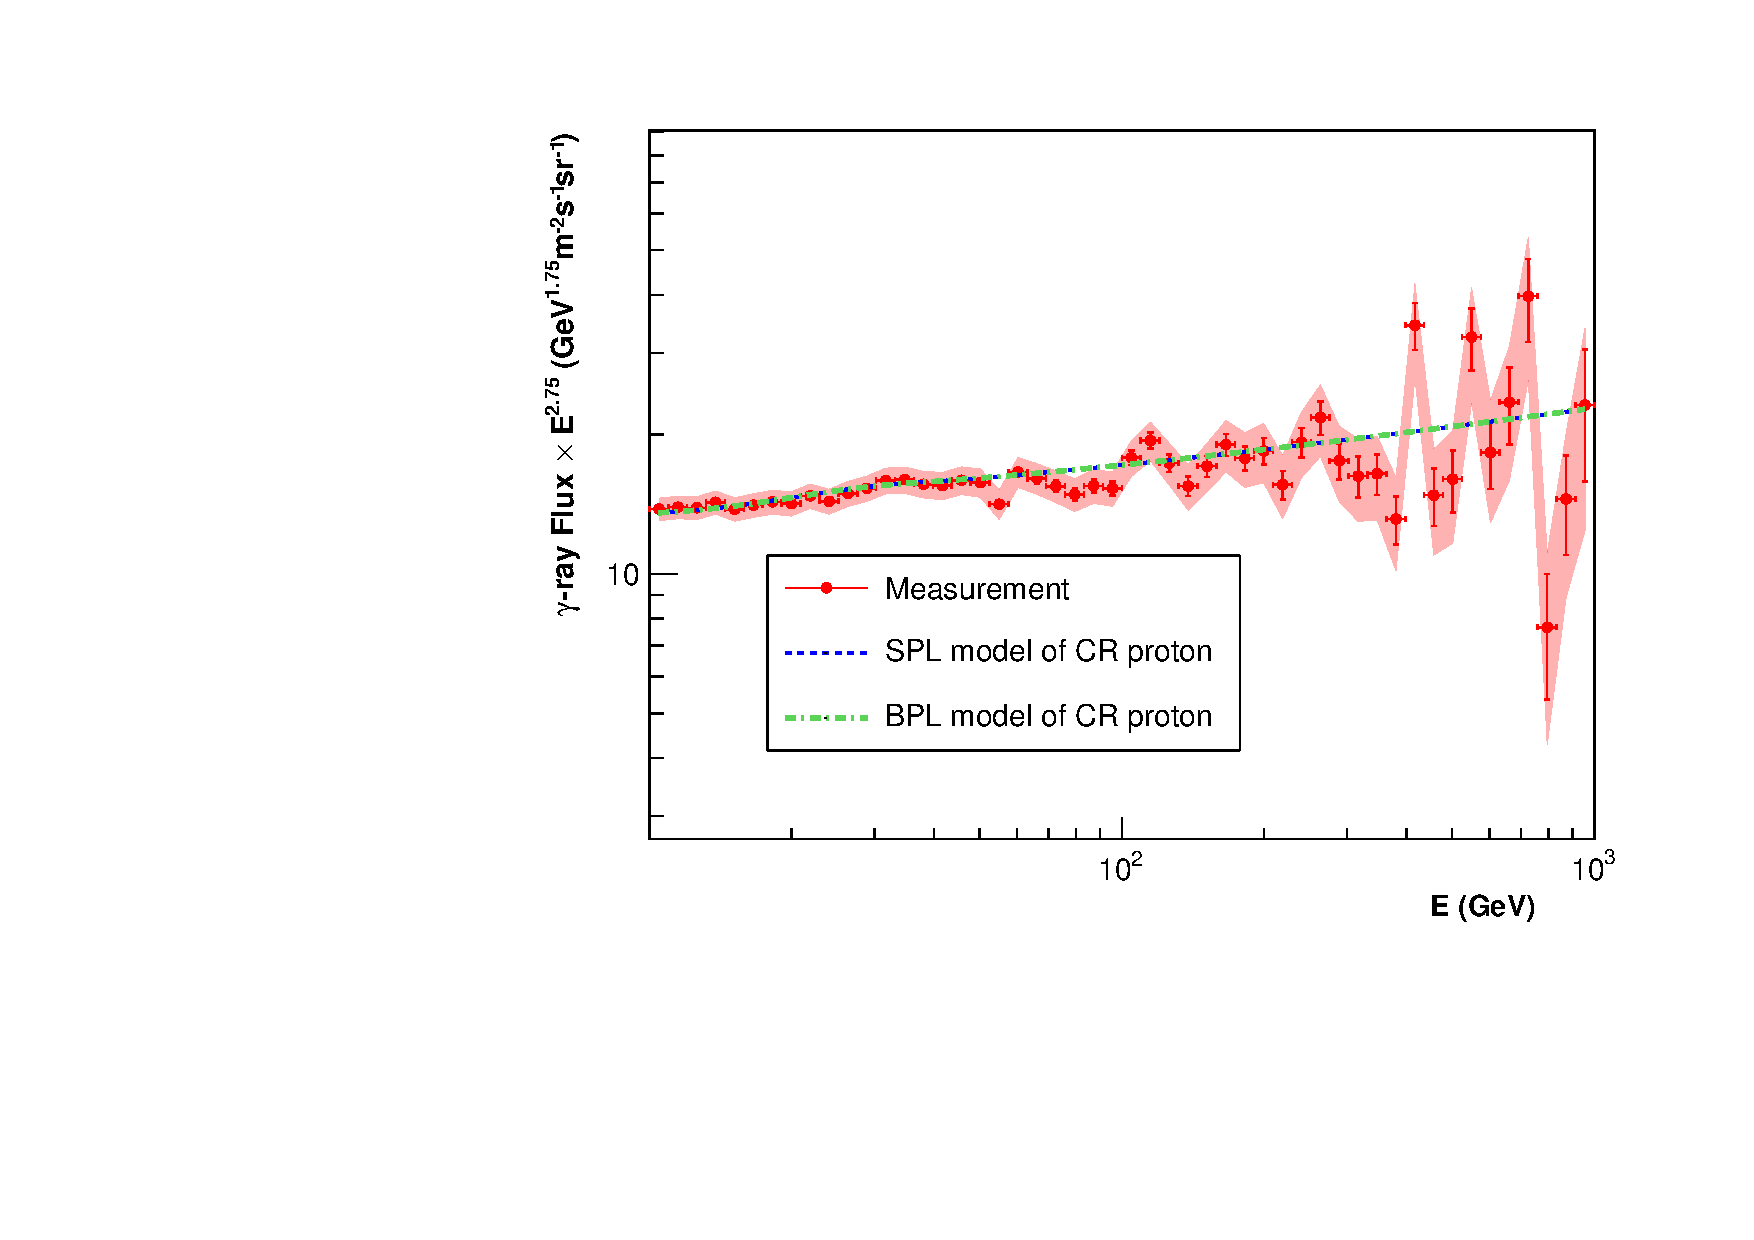
\includegraphics[width=0.8\textwidth]{content/result_and_discussion/figures/fitted_result.pdf}
    \caption{
        The $\gamma$-ray spectra calculated from the SPL (red)
        and BPL (blue) models of CR proton which best fit with the
        measured Earth's $\gamma$-ray spectrum in the thin-target
        regime (red).
    }
    \label{fig:fitted_gamma_specgtrum}
\end{figure}

\newpage 

\begin{figure}[h!]
    \centering
    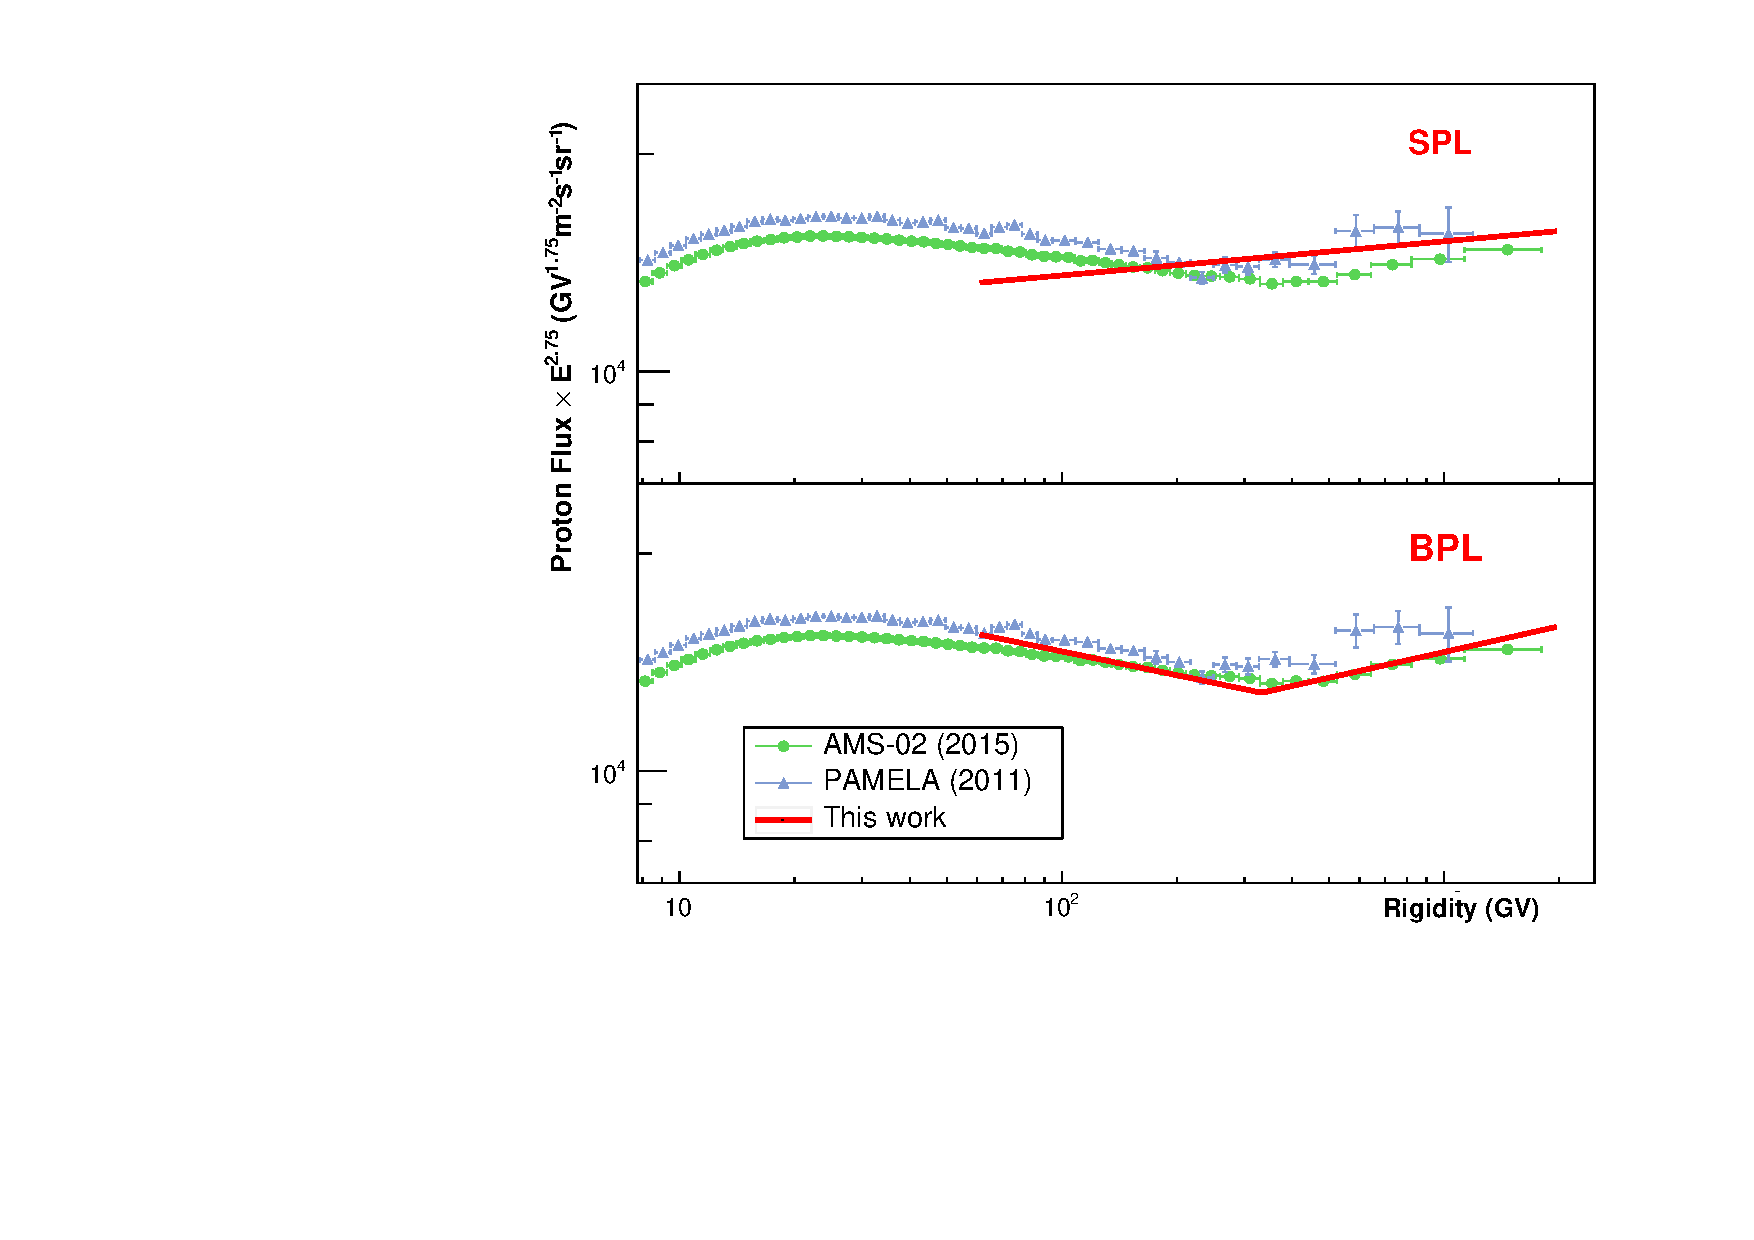
\includegraphics[width=0.9\textwidth]{content/result_and_discussion/figures/ProtonSpectrumModelMeasurement.pdf}
    \caption{
        Best-fit CR proton spectrum from this work (red)
        compared to the measurementsby AMS-02 (blue) and
        PAMELA (green).
    }
    \label{fig:fitted_cr_proton}
\end{figure}





% \lofcont

\chapter{Conclusion}

example cite \cite{curie1923pierre}


\nocite{*}

\bibliographystyle{muthesis}
%\bibliography{abbrev,mbib,conf} % for bibtex (recommended!!!)
%\bibliographystyle{plainnat}

%\bibliography{mybirds_0}
\bibliography{JABTHESISBIB}
%\bibliography{Busbib}
%\bibliography{paper}

%\input{fhoonethesis_bib.tex}



\appendices


\chapter{Testing the exposure map}
\label{appendix:exposure}
..

\chapter{Power law in energy}
\label{appendix:pw_energy}


\chapter{Subtracting $\gamma$-ray background}
blabla

\chapter{Interaction Model}
\label{appendix:interaction_model}


% \chapter{Count Map Transformation}{\label{countmapcode}}

% We transform the positions of arriving photons into the geographical coordinate system (latitude and longtitude). The parameters used in the transformation are defined in Figure~\ref{fig:mesh}. The \tca{$R$} represents the radius of Earth. The $h_{s}$ and $h_{p}$ denote the height of $\textit{Fermi}$ and the $\gamma$-ray production altitude, respectively.

% \begin{figure}[h]
%     \centering
%     \includegraphics[width=0.5\textwidth]{Parameters.eps}
%     \caption{Definitions of parameters used in the coordinate transformation.}
%     \label{fig:mesh}
% \end{figure}


% \noindent \textbf{Strategy} ::  
% \tca{Consider three Earth-centered coordinate systems:} 
% \begin{itemize}[labelindent=\parindent, leftmargin=0pt,itemindent=*, itemsep=0pt, topsep=0pt]
% \item{First use ``primed" \tca{coordinates} with pole toward {\it Fermi} and relate the angles of the $\gamma$ incidence to the coordinates of $\gamma$ emission}
% \item{ Then rotate to ``starred" \tca{coordinates} with pole to North pole and \textit{Fermi} at longitude 180$^{\circ}$ and desired \tca{latitude} ($\varphi$) }
% \item{Then rotate \textit{Fermi} to desired longitude ($\lambda$) to determine the final coordinates of $\gamma$ emission}
% \end{itemize}

% \newpage

% \begin{itemize}[labelindent=\parindent, leftmargin=0pt,itemindent=*, itemsep=0pt, topsep=0pt]
% \item\textbf{View the system of  \textit{Fermi} over the pole of ``primed coordinate"}
% \end{itemize}


% \indent \tca{At first, we know the measured $\Theta_{\rm Nad}$ and assume that we know $h_p$. We want to determine the angular displacement $\theta'$ of the photon's geographic point of origin relative to \textit{Fermi}'s angular position. First we find the lateral displacement $x$ in terms of $\Theta_{\rm Nad}$.} Starting with \tca{a} right triangle, 
% \begin{eqnarray}
% x^{2} + z^{2} & = & R'^{2}\tca{,}  \nonumber
% \end{eqnarray}
% \noindent where
% \begin{eqnarray}
% x  & =  & (R'+h'-z)\tan \mathrm{\Theta_{\rm Nad}} \nonumber \\ 
% z  & = & R'+h'-x\cot \mathrm{\Theta_{\rm Nad}}. \nonumber
% \end{eqnarray}
% \noindent So that,
% \begin{eqnarray}
% x^{2} +(R'+h')^{2} -2x(R'+h') \cot \mathrm{\Theta_{\rm Nad}} +x^{2} \cot ^{2}\mathrm{\Theta_{\rm Nad}} & = & R'^{2}  \nonumber \\
% (1+\cot ^{2}\mathrm{\Theta_{\rm Nad}}) x^{2} -2x(R'+h') \cot \mathrm{\Theta_{\rm Nad}} + (R' + h')^{2} - R'^{2} & = & 0  \nonumber \\
% x^{2} \csc^{2}\mathrm{\Theta_{\rm Nad}} - 2x(R'+h')\cot \mathrm{\Theta_{\rm Nad}} + (2h'R' +h'^{2}) & = & 0 \nonumber \\
% x^{2} - 2x(R'+h')\sin \mathrm{\Theta_{\rm Nad}} \cos \mathrm{\Theta_{\rm Nad}} + (2h'R'+h'^{2})\sin^{2}\mathrm{\Theta_{\rm Nad}} & = & 0.  \nonumber
% \end{eqnarray}
% \noindent Solving quadratic equations,
% \begin{eqnarray}
% x & = & \frac{1}{2}\Big[2(R'+h')\sin \mathrm{\Theta_{\rm Nad}} \cos \mathrm{\Theta_{\rm Nad}}  \nonumber \\
% &  & \pm \sqrt{4(R'+h')^{2}\sin^{2}\mathrm{\Theta_{\rm Nad}} \cos^{2}\mathrm{\Theta_{\rm Nad}} -4(2h'R'+h'^{2})\sin^{2}\mathrm{\Theta_{\rm Nad}}}\Big]. \nonumber 
% \end{eqnarray}
% \noindent We want first intersection of incidence, so use ``-" sign
% \begin{eqnarray}
% x & = & (R'+h')\sin \mathrm{\Theta_{\rm Nad}} \cos\mathrm{\Theta_{\rm Nad}}  \nonumber \\
%   &  & - \sin \mathrm{\Theta_{\rm Nad}} \sqrt{(R'+h')^{2} \cos^{2}\mathrm{\Theta_{\rm Nad}} -2h'R'-h'^{2}}.\nonumber
% \end{eqnarray}
% \noindent Thus,
% \begin{eqnarray}
% \sin \theta' & =& \frac{x}{R'} \nonumber \\
% \sin \theta' & = & \sin\mathrm{\Theta_{\rm Nad}} \bigg[\Big(1+\frac{h'}{R'}\Big)\cos\mathrm{\Theta_{\rm Nad}} \nonumber \\
% & & - \sqrt{\Big(1+\frac{h'}{R'}\Big)^{2}\cos^{2}\mathrm{\Theta_{\rm Nad}} -2\frac{h'}{R'}-\Big(\frac{h'}{R'}\Big)^{2}}\bigg]. \nonumber
% \end{eqnarray}
% \tca{As a check, note that $\Theta_{\rm Nad}=0^{\circ}$ implies $\theta'=0^{\circ}$, as it should.} 

% \begin{itemize}[labelindent=\parindent, leftmargin=0pt,itemindent=*, itemsep=0pt, topsep=0pt]
% \item\textbf{In primed coordinates (with the pole toward \textit{Fermi})}
% \end{itemize}

% \noindent \textit{Fermi} :: $x'_{F} = y'_{F} =0$,  $z'_{F}=R+h_{s}$ \\
% $\gamma$-ray emission point :: $x'=R'\sin\theta' \cos\Phi_{\rm Zen}$, $y'=R'\sin\theta' \sin \Phi_{\rm Zen}$,  $z' = R'\cos\theta'$ \\  

% \indent We will now rotate to star\tca{r}ed coordinates, in which \textit{Fermi} is at latitude $\varphi$ (desired latitude) and longitude 180$^{\circ}$. The reason for longitude 180$^{\circ}$  is so that the azimuth\tca{al angle $\Phi_{\rm Zen}=0^{\circ}$} corresponds to arrival from N.
% \begin{eqnarray}
% x^{*} & = & \cos \Theta x'-\sin \Theta z' \nonumber \\
% y^{*} & = & y' \nonumber \\
% z^{*} & = & \sin \Theta x' + \cos \Theta z' \nonumber 
% \end{eqnarray}
% \begin{figure}[h]
%     \centering
%     \includegraphics[width=0.8\textwidth]{prime}
%     \caption{\tca{The primed and starred coordinates} ($z^{*}$ is \tca{along} North pole)}
%     \label{fig:mesh1}
% \end{figure}
% \begin{eqnarray}
% x^{*} & = & \sin \varphi x'-\cos \varphi z' \nonumber \\
% y^{*} & = & y' \nonumber \\
% z^{*} & = & \cos \varphi x' + \sin \varphi z' \nonumber 
% \end{eqnarray}
% \noindent \textbf{Check :: } Where does \textit{Fermi} move to?
% \begin{eqnarray}
% x^{*} & = &  \tca{-}(R+h_{s})\cos \varphi \nonumber \\
% y^{*} & = & 0 \nonumber \\
% z^{*} & = & (R+h_{s}) \sin \varphi  \nonumber 
% \end{eqnarray}
% \noindent $\gamma$-ray emission point :: 
% \begin{eqnarray}
% x^{*} & = & R'(\sin \theta' \cos \Phi_{\rm Zen} \sin \varphi - \cos \theta' \cos \varphi ) \nonumber \\
% y^{*} & = & R'(\sin \theta' \sin \Phi_{\rm Zen}) \nonumber \\
% z^{*} & = & R'(\sin \theta' \cos \Phi_{\rm Zen} \cos \varphi + \cos \theta' \sin \varphi) \nonumber  \\
% x^{*2} + y^{*2} + z^{*2} & = & R'^{2} \nonumber
% \end{eqnarray}

% \begin{itemize}[labelindent=\parindent, leftmargin=0pt,itemindent=*, itemsep=0pt, topsep=0pt]
% \item\textbf{Our desired coordinates::}
% Rotate so that \textit{Fermi}\tca{'s equatorial projection} move\tca{s} from $-x^{*}_{F}$ direction to longitude $\lambda$ (E of primed meridian) \tca{from} $+x$
% \end{itemize}

% \begin{figure}[h]
%     \centering
%     \includegraphics[width=0.6\textwidth]{desired}
%     \caption{\tca{The unprimed and starred coordinates. The satellite is depicted at its equatorial projection.}}
%     \label{fig:mesh1}
% \end{figure}
% \begin{eqnarray}
% x & = & -\cos \lambda x^{*} + \sin \lambda y^{*} \nonumber \\
% y & = & - \sin \lambda x^{*} - \cos \lambda y^{*} \nonumber \\
% z & = & z^{*} \nonumber 
% \end{eqnarray}
% \textbf{Check :: } Where does \textit{Fermi} move to?
% \begin{eqnarray}
% x_{F} & = & (R+h_{s})\cos \varphi \cos \lambda \nonumber \\
% y_{F} & = & (R+h_{s})\cos \varphi \sin \lambda  \nonumber \\
% z_{F} & = & (R+h_{s}) \sin \varphi  \nonumber 
% \end{eqnarray}
% \noindent $\gamma$-ray emission point :: 
% \begin{eqnarray}
% x & = & R'(- \sin \theta' \cos \Phi_{\rm Zen} \sin \varphi \cos \lambda + \sin \theta' \sin \Phi_{\rm Zen} \sin \lambda \nonumber \\
% & & + \cos \theta' \cos \varphi \cos \lambda ) \nonumber \\
% y & = & R'(- \sin \theta' \cos \Phi_{\rm Zen} \sin \varphi \sin \lambda - \sin \theta' \sin \Phi_{\rm Zen} \cos \lambda  \nonumber \\
% & & + \cos \theta' \cos \varphi \sin \lambda ) \nonumber \\
% z & = & R'( \sin \theta' \cos \Phi_{\rm Zen} \cos \varphi + \cos \theta' \sin \varphi) \nonumber \\
% x^{2}+y^{2}+z^{2} & = & R'^{2}\big([(-\sin \theta' \cos \Phi_{\rm Zen} \sin \varphi + \cos\theta' \cos \varphi)^{2}  \nonumber \\
% & & + (\sin\theta' \sin\Phi_{\rm Zen})^{2}] \cos^{2}\lambda + [\sin^{2} \theta' \sin^{2} \Phi_{\rm Zen} \nonumber \\
% &  &  + (-\sin \theta' \cos \Phi_{\rm Zen} \sin \varphi + \cos \theta' \cos \varphi)^{2}]\sin^{2} \lambda \nonumber \\
% & & + (\sin \theta' \cos \Phi_{\rm Zen} \cos \varphi + \cos \theta' \sin \varphi)^{2}\big) \nonumber \\
% & = & R'^{2}[(-\sin \theta' \cos \Phi_{\rm Zen} \sin \varphi + \cos \theta' \cos \varphi)^{2} + \sin^{2} \theta' \sin^{2} \Phi_{\rm Zen} \nonumber \\
% &  & + (\sin \theta' \cos \Phi_{\rm Zen} \cos \varphi + \cos \theta' \sin \varphi)^{2}] \nonumber \\
% & = & R'^{2}[\sin^{2}\theta' \cos^{2} \Phi_{\rm Zen} \sin^{2} \varphi -2\sin \theta' \cos \theta' \cos \Phi_{\rm Zen} \sin \varphi \cos \varphi  \nonumber \\
% & & + \cos^{2}\theta' \cos^{2}\varphi + \sin^{2}\theta' \sin^{2}\Phi_{\rm Zen} + \sin^{2}\theta' \cos^{2} \Phi_{\rm Zen} \cos^{2} \varphi  \nonumber \\
% & & + 2\sin \theta' \cos \theta' \cos \Phi_{\rm Zen} \sin \varphi \cos \varphi \nonumber + \cos^{2}\theta' \sin^{2}\varphi ] \nonumber  \\
% & =&  R'^{2}[\sin^{2}\theta' \cos^{2} \Phi_{\rm Zen} (\sin^{2} \varphi+\cos^{2}\varphi) + \sin^{2}\theta' \sin^{2}\Phi_{\rm Zen} \nonumber \\
% & & +\cos^{2}\theta' (\cos^{2}\varphi+\sin^{2}\varphi) ]\nonumber  \\
% & = &  R'^{2}[\sin^{2}\theta' ( \cos^{2} \Phi_{\rm Zen} + \sin^{2}\Phi_{\rm Zen} )+\cos^{2}\theta' ] \nonumber  \\
% & =& R'^{2} \nonumber 
% \end{eqnarray}
% \noindent If $\theta' = 0^\circ $, $\gamma$ \tca{is} from \tca{the} nadir \tca{and} should \tca{come from the same direction as} \textit{Fermi} \tca{but from} Radius $R'$, \tca{and indeed} 
% \begin{eqnarray}
% x & = & R'(\cos \varphi \cos \lambda) \nonumber \\
% y & = & R'(\cos \varphi \sin \lambda) \nonumber \\
% z & = & R' \sin \varphi \nonumber \\
% x^{2}+y^{2}+z^{2} & = & R'^{2}[\cos^{2} \varphi (\cos^{2}\lambda + \sin^{2}\lambda) + \sin^{2} \varphi ]  \nonumber \\
% & = & R'^{2} \nonumber 
% \end{eqnarray}

% \noindent \noindent \textbf{\tca{Latitude} and Longitude of $\gamma$ emission ($\varphi_{\gamma}$, $\lambda_{\gamma}$)}
% \begin{eqnarray}
% \sin \varphi_{\gamma} & = \tca{\frac{z}{R'}} & = \sin \theta' \cos\Phi_{\rm Zen} \cos \varphi + \cos \theta' \sin \varphi \nonumber \\
% \cos \varphi_{\gamma} \cos \lambda_{\gamma} & = \tca{\frac{x}{R'}} & = - \sin \theta' \cos \Phi_{\rm Zen} \sin \varphi \cos \lambda + \sin \theta' \sin \Phi_{\rm Zen} \sin \lambda  \nonumber \\
%  & = & + \cos \theta' \cos \varphi \cos \lambda \nonumber \\
% \cos \varphi_{\gamma} \sin \lambda_{\gamma} & = \tca{\frac{y}{R'}} & = - \sin \theta' \cos \Phi_{\rm Zen} \sin \varphi \sin \lambda - \sin \theta' \sin \Phi_{\rm Zen} \cos \lambda \nonumber \\
% & = & + \cos \theta' \cos \varphi \sin \lambda .  \nonumber
% \end{eqnarray}


% \chapter{Exposure Map Transformation}{\label{exposuremapcode}}


% \indent The exposure map is computed by integrating\tca{, for 10 years of data that I analyze,} the \tcb{effective area, livetime, and solid} angle product over the same geographical \tca{coordinate} grid as the counts map, taking into account the changing orientation of the LAT and the corrections for rate-dependent inefficiency.  The latter takes into account the loss of effective area in regions of the {\it Fermi} orbit where the rate of charged-particle background interaction with the LAT is high. \tcb{For a given pixel,}

% \begin{eqnarray}
% \textnormal{Exposure} =   A_{\mathrm{eff}}(E,\theta,\phi)\cdot\textnormal{livetime}\cdot\textnormal{solid angle} \label{eq1}
% \end{eqnarray}
% where\\
% \indent $E$ is energy for different incoming photons in MeV \\
% \indent $\theta$ is the angle \tca{of} a pixel (in the geographical coordinates) relative to the LAT's boresight ($z$-axis of spacecraft) as shown in Figure \ref{fig:LATcoordinate}  \\
% \indent $\phi$ is the angle \tca{of the projection of} a pixel (in the geographical coordinates) \tca{perpendicular to the boresight,} relative to the $x$-axis of \tca{the} spacecraft as shown in Figure \ref{fig:LATcoordinate}  \\
% \indent \tcb{livetime} is the time that the LAT observed a given position \\
% \indent \tca{solid angle is the direction dependent} solid angle per pixel in gepgraphical longitude and latitude.

% \begin{figure}[h!]
%     \centering
%     \includegraphics[width=0.9\textwidth]{Coordinatesystem.png}
%     \caption{Red arrow \tca{($\vec{V}'$)} represents a vector \tca{from \textit{Fermi}} in the equatorial ($x'y'z'$) coordinate system pointing toward a pixel of interest in the geographical coordinates. }
%     \label{fig:LATcoordinate}
% \end{figure}

% \begin{itemize}[labelindent=\parindent, leftmargin=0pt,itemindent=*, itemsep=0pt, topsep=0pt]
% \item\textbf{\tca{Coordinate transformation}}
% \end{itemize}

% Here, Equation \ref{eq3} -- \ref{eq5} are used to evaluate the exposure maps as defined in Equation~\ref{eq1}. Rotation and translation matrices for transformation between two coordinate systems, the geographical ($xyz$) and equatorial ($x'y'z'$) as illustrated in Figure~\ref{fig:Coordinate}, are given in Equation~\ref{eq2}. Note that $z$ and $z'$ axes \tca{are in} the same \tca{direction} at all times. The transformation equations can be written as

% \[
% \begin{bmatrix}
%     x'    \\
%     y'    \\
%     z'    \\
% \end{bmatrix}
% =
% \begin{bmatrix}
%     \textnormal{cos}\alpha & -\textnormal{sin}\alpha & 0\\
%     \textnormal{sin}\alpha & \textnormal{cos}\alpha  & 0\\
%     0 & 0 & 1 \\
% \end{bmatrix}
% \begin{bmatrix}
%     x  \\
%     y  \\
%     z  \\ 
% \end{bmatrix}
% +
% \begin{bmatrix}
%     \Delta x'  \\
%     \Delta y'  \\
%     \Delta z'  \\ 
% \end{bmatrix}
% \]  

% \begin{equation}
% \vec{V}' = \begin{cases}
% x'  =   x \cos \alpha - y \sin \alpha + \Delta x' \\ \label{eq2}
% y'  =   x \sin \alpha - y \cos \alpha + \Delta y' \\
% z'  =   z + \Delta z' 
% \end{cases}
% \end{equation}

% \noindent where\\
% \indent $\alpha$ is rotated angle as shown in Figure  \ref{fig:Coordinate}  \\
% \indent $x$ points to the Prime Meridian along the equatorial plane (longitude = 0$^\circ$) \\ 
% \indent $y$ is orthogonal to both $x$ and $z$ according to the right-hand rule \\
% \indent $z$ points toward the north polar axis \\
% \indent $x'$ points toward the vernal equinox (RA = 0$^\circ$) \\
% \indent $y'$ is orthogonal to $x'$ and $z'$ \\
% \indent $z'$ points to the North celestial pole \\
% \indent \tca{$\Delta x'$, $\Delta y'$, and $\Delta z'$ are \tcb{the coordinates of the origin of the $xyz$ frame measured in the $x'y'z'$ frame}.}

% \begin{figure}[h!]
%     \centering
%     \includegraphics[width=0.4\textwidth]{Coordinate}
%     \caption{The definition of the rotation angle $\alpha$. }
%     \label{fig:Coordinate}
% \end{figure}
% \begin{itemize}[labelindent=\parindent, leftmargin=*]
% \item\textbf{\tca{Determining $\cos\alpha$ and \tcb{$\sin\alpha$}}}
% \end{itemize}

% \indent In each time step, there is a point directly below the LAT which is recorded in both geographical (latitude and longitude of the LAT's ``\tca{projection}'' on the Earth's surface) and equatorial (RA and DEC of the LAT's nadir direction) \tcb{angles}. \tcb{Using the Earth's radius and spacecraft's altitude, W}e can easily determine the coordinates of this point in the two coordinate systems, say ($x_0,y_0,z_0$) and ($x'_0,y'_0,z'_0$) respectively, and use them to calculate $\cos \alpha$ and $\sin \alpha$ as follows.
% \begin{eqnarray}
%  x'_0 - \Delta x'_0 & = & x_0 \textnormal{cos}\alpha - y_0 \textnormal{sin}\alpha \label{eq3} \\
%  y'_0 - \Delta y'_0 & = & x_0 \textnormal{sin}\alpha + y_0 \textnormal{cos}\alpha \label{eq4}  \\
% \textnormal{\ref{eq3}} \times x_0 ;  (x'_0 - \Delta x'_0)x_0 & = & x_0^{2} \textnormal{cos}\alpha - x_0y_0 \textnormal{sin}\alpha \\
% \textnormal{\ref{eq4}} \times y_0;  (y'_0 - \Delta y'_0)y_0 & = & x_0y_0 \textnormal{sin}\alpha + y_0^{2} \textnormal{cos}\alpha \\
%  \textnormal{cos}\alpha & = & \frac{[(x'_0 -  \Delta x'_0)x_0 + (y'_0 - \Delta y'_0 )y_0]}{(x_0^{2} + y_0^{2})} \\
% \textnormal{\ref{eq3}} \times y_0 ; (x'_0 - \Delta x'_0)y_0 & = & x_0y_0\textnormal{cos}\alpha - y_0^{2}\textnormal{sin}\alpha \\
% \textnormal{\ref{eq4}} \times y_0 ; (y'_0 - \Delta y'_0)x_0 & = & x_0^{2}\textnormal{sin}\alpha + x_0y_0\textnormal{cos}\alpha \\
%  \textnormal{sin}\alpha & = & \frac{[(y'_0 -  \Delta y'_0)x_0 + (x'_0 - \Delta y'_0)x_0]}{(x_0^{2} + y_0^{2})} 
% \end{eqnarray}
% \tcb{We can also extend the vector ($x'_0,y'_0,z'_0$) to length $R+h_s$ to determine ($\Delta x'$,$\Delta y'$,$\Delta z'$).}

% \clearpage 

% \begin{itemize}[labelindent=\parindent, leftmargin=0pt,itemindent=*, itemsep=0pt, topsep=0pt]
% \item\textbf{\tca{Using $\vec{V}'$ for a pixel to determine $\theta$ and $\phi$}}
% \end{itemize}

% In each time step during observation, the LAT's orientation can be defined by its $z$-axis pointing along its boresight, and its $x$-axis pointing along one of its solar panel. They are $z_{\rm s}$ and $x_{\rm s}$ in Figure~\ref{fig:LATcoordinate}. The direction of the LAT's $z_{\rm s}$ and $x_{\rm s}$ recorded in the FT2 files are referred to as (RAZ, DEZ) and (RAX, DEX) respectively. The unit vector components of $z_{\rm s}$ in the equatorial frame can be written as

% \begin{equation}
% \vec{V}_{z} = \begin{cases}
% x_{z}  =  \cos(\textnormal{DEZ})\cos(\textnormal{RAZ})  \\
% y_{z}  =  \cos(\textnormal{DEZ})\sin(\textnormal{RAZ})  \\
% z_{z}  =  \sin(\textnormal{DEZ}) 
% \end{cases}
% \end{equation}

% \noindent and those of the LAT's x-axis are

% \begin{equation}
% \vec{V}_{x} = \begin{cases}
% x_{x}  =  \cos(\textnormal{DEX})\cos(\textnormal{RAX})  \\
% y_{x}  =  \cos(\textnormal{DEX})\sin(\textnormal{RAX})  \\
% z_{x}  =  \sin(\textnormal{DEX}).
% \end{cases}
% \end{equation}

% So, $\vec{V}_{y}$ is the cross product of two vectors ($\vec{V}_{z}$ $\times$ $\vec{V}_{x}$) which is given by the formula,
% \begin{equation}
%  \vec{V}_{z} \times \vec{V}_{z}=
%    \begin{vmatrix} 
%     \hat{i} & \hat{j} & \hat{k} \\
%     x_{z} & y_{z} & z_{z} \\
%     x_{x} & y_{x} & z_{x} \\
%    \end{vmatrix} 
% \end{equation}

% \noindent Then, 
% \begin{equation}
% \vec{V}_{y} = \begin{cases}
% x_{y}  =  y_{z}z_{x} - y_{x}z_{z} \\
% y_{y}  =  x_{x}z_{z} - x_{z}z_{x} \\
% z_{y}  =  x_{z}y_{x} - x_{x}y_{z} 
% \end{cases}
% \end{equation}

% \tca{For any pixel of interest, we know \tcb{($x$, $y$, $z$)} and can use Equation \ref{eq2} to calculate \tcb{$\vec{V}' = (x',y',z')$}.} \tcb{Therefore}, $\theta$ and $\phi$ can be calculated by
% \begin{eqnarray}
% \theta & = & \cos^{-1} \Big( \frac{A_{z}}{A_{t}} \Big)  \\
% \phi & = & \tan^{-1} \Big( \frac{A_{y}}{A_{x}} \Big)   \label{eq5}
% \end{eqnarray}
% \noindent where\\
% \indent\indent $A_{x}$ is the product of $\vec{V}' \cdot \vec{V}_{x}$ \\ 
% \indent\indent $A_{y}$ is the product of $\vec{V}' \cdot \vec{V}_{y}$ \tca{for} ($\vec{V}_{y}$ = $\vec{V}_{z} \times \vec{V}_{x}$)\\
% \indent\indent $A_{z}$ is the product of $\vec{V}' \cdot \vec{V}_{z}$ \\ 
% \indent\indent $A_{t}$ = $\sqrt{A_{x}^{2}+A_{y}^{2}+A_{z}^{2}}$ = $|\vec{V}'|$.  \\

% \begin{itemize}[labelindent=\parindent, leftmargin=0pt,itemindent=*, itemsep=0pt, topsep=0pt]
% \item\textbf{\tca{Solid angle calculation}}
% \end{itemize}
% \begin{figure}[h!]
%     \centering
%     \includegraphics[width=0.6\textwidth]{solidangle}
%     \caption{Drawing of vectors \tcb{which are} used in solid angle estimation. }
%     \label{fig:Solidangle}
% \end{figure}

% \tca{Solid angle ($\Omega$) \tcb{is defined} as an area on the surface of \tcb{a unit sphere} centered at the vertex of the angle.} \tcb{The SI unit of $\Omega$ is steradian (sr).} In this work, $\Omega$ \tcb{is the solid angle size of a pixel of interest in the geographical map as observed by the LAT at a given time}. We estimate the $\Omega$ from \tcb{the tetrahedron $OABC$ as shown in Figure~\ref{fig:Solidangle}} with an origin at point $O$ \tcb{and} $\vec{a}$, $\vec{b}$, $\vec{c}$ represent the vectors from $O$ to vertices $A$, $B$, and $C$\tcb{, respectively, using a formula given by \cite{solidangle}}.

% \begin{eqnarray}
% \tan\bigg( \frac{1}{2}\Omega \bigg) = \frac{\vec{a}\cdot(\vec{b}\times\vec{c})}{abc + (\vec{a}\cdot\vec{b})c + (\vec{b}\cdot\vec{c})a + (\vec{c}\cdot\vec{a})b}
% \end{eqnarray}
% \tcb{\noindent where $a$, $b$, and $c$ are the magnitude of $\vec{a}$, $\vec{b}$, and $\vec{c}$, respectively.}
% \tcb{The solid angle size of this pixel is the sum of the the solid angle subtended by the triangular face $ABC$ and $ACD$.}


\biography

\end{document}

